\chapter{Experiment}
\label{expr}

Aby bylo možné porovnat stávající řešení s nově navrženým řešením na poli rychlosti zpracovávání dotazů a ověřit naše předpoklady, podrobili jsme zmíněná řešení experimentu. 
Vykonaný experiment proběhne na reálných grafech různé velikosti s uměle vygenerovanými vlastnostmi naležící vrcholům. 
Nad danými grafy provedeme vybrané množství dotazů, které nám umožní sledovat a porovnat chování řešení v různých situacích.
Experiment bude zakončen diskuzí nad výsledky. 

\section{Příprava dat}
\label{expr.graphs}

Pro náš experiment jsme použili tři orientované grafy z databáze SNAP\footnote{\citet{snapnets}}.

\begin{table}[!htb]
\centering
\begin{tabular}{lrr}
\toprule
\mc{} & \mc{\textbf{\#Vrcholů}} & \mc{\textbf{\#Hran}} \\
\midrule
Amazon0601     & 403394 & 3387388 \\
WebBerkStan & 685230   & 7600595 \\
As-Skitter    & 1696415   & 11095298 \\
\bottomrule
\end{tabular}

\caption{Vybrané grafy pro experiment}
\label{tab.grafBase}
\end{table}

\begin{itemize}

\item \textbf{Amazon0601:} Jedná se o graf vytvořený procházením webových stránek Amazonu na základě featury „Customers Who Bought This Item Also Bought“ ze dne 1.6.2003. V grafu existuje hrana z $i$ do $j$, pokud je produkt $i$ často zakoupen s produktem $j$.

\item \textbf{WebBerkStan:} Graf popisuje odkazy webových stránek domén \url{https://www.stanford.edu/} a \url{https://www.berkeley.edu/}. Vrcholem je webová stránka a hrana představuje hypertextový odkaz mezi stránkami.

\item \textbf{As-Skitter:} Topologický graf internetu z roku 2005 vytvořený programem \verb+traceroutes+. Ačkoliv je uvedeno, že daný graf je neorientovaný, vnitřní hlavička souboru uvádí opak, proto jsme se daný graf rozhodli přesto využít.

\end{itemize}

Samotné grafy obsahují pouze seznam hran. Abychom mohli dané grafy využít, bylo nutné je transformovat a vygenerovat k nim Properties na vrcholech. 
Při příkladu transformace budeme vycházet z následující ukázky hlavičky (graf Amazon0601):

\begin{code}
# Directed graph (each unordered pair of nodes is saved once): 
    Amazon0601.txt: 
# Amazon product co-purchaisng network from June 01 2003
# Nodes: 403394 Edges: 3387388
# FromNodeId	ToNodeId
0	1
0	2
0	3
0	4
\end{code}

\subsection{Transformace grafových dat}

Výstupem transformace budou soubory popisující schéma vrcholů/hran NodeTypes.txt/EdgeTypes.txt a datové soubory vrcholů/hran Nodes.txt/Edges.txt.
V našem případě graf bude obsahovat pouze jeden typ hrany a jeden typ vrcholu. 
Dané omezení pouze snižuje počet nalezených výsledků, což není určující pro náš experiment. 

Ukázka zvoleného schématu pro Nodes.txt/Edges.txt:
\begin{code}
Soubor EdgeTypes.txt:
[
{ "Kind": "BasicEdge" }
]

Soubor NodeTypes.txt:
[ 
{ "Kind": "BasicNode" }
]

\end{code}

Generování souborů Edges.txt/Nodes.txt provádí program, který je obsahem přílohy zdrojových kódů \ref{prilohy.kod} v souboru GrapDataBuilder.cs.
Výstupní soubor Edges.txt bude obsahovat hrany v rostoucím pořadí dle položky \verb+FromNodeId+ z originálního souboru s přidělenými \verb+IDs+ od hodnoty \verb+ID+ posledního vrcholu v souboru Nodes.txt.
Samotný soubor Nodes.txt obsahuje setřiděné vrcholy podle \verb+ID+ v rostoucím pořadí. Je nutné zmínit, že setřídění dat podle \verb+ID+ není nežádoucí, jelikož nezaručuje nic o seskupení vrcholů v daném grafu.
Pro připomenutí zmíníme, že prvni sloupeček v datových souborech Edges.txt a Nodes.txt odpovídá unikátnímu \verb+ID+ v rámci celého grafu.

Následuje ukázka výstupních souborů transformace pro graf Amazon0601:  
\begin{code}
Soubor Edges.txt:
403395 BasicEdge 0 1
403396 BasicEdge 0 2
...

Soubor Nodes.txt:
0 BasicNode 
1 BasicNode 
...
\end{code}

\subsection{Generování Properties vrcholů}

Posledním krokem přípravy dat pro experiment je vygenerování Properties vrcholů.
Jsme si vědomi, že nejideálnější způsob testování je graf s reálnými daty. Nicméně, dané omezení jsme se rozhodli aplikovat kvůli problematickému hledání vhodných dat, které nevyžadují netriviální transformaci do vhodného vstupního formátu.
Proto pro každý vrchol náhodně vygenerujeme hodnoty čtyř Properties. 
\clearpage
\begin{table}[!htb]
\centering
\begin{tabular}{llll}
\toprule
\mc{\textbf{Property}} & \mc{\textbf{Type}}  & \mc{\textbf{Popis}}\\
\midrule
PropOne     & integer &  \verb+Int32+ s rozsahem $[0; 100000]$ \\
PropTwo & integer   & \verb+Int32+ s rozsahem $[$\verb+Int32.MinValue+; \verb+Int32.MaxValue+$]$ \\
PropThree    & string &  délka $[2; 8]$ ASCII znaků s rozsahem $[33; 126]$ \\
PropFour & integer   & \verb+Int32+ s rozsahem $[0; 1000]$ \\
\bottomrule
\end{tabular}

\caption{Generované Properties vrcholů}
\label{tab.grafProps}
\end{table}

\begin{itemize}

\item \textbf{PropTwo} hodnoty jsou rovněž generováný střídavě kladně a záporně, aby nastal rovnoměrný počet záporných a kladných hodnot.

\item \textbf{PropThree} hodnoty jsou pouze ASCII znaky z rozsahu $[33; 126]$. Dané omezení výplývá z vlastností dotazovacího enginu, aby bylo možné bez obtíží načíst datový soubor.

\end{itemize}

Na základě tabulky generovaných Properties \ref{tab.grafProps} následuje ukázka upraveného souboru schématu pro vrcholy:
\begin{code}
Soubor NodeTypes.txt:
[
{ 
"Kind": "BasicNode",
"PropOne": "integer",
"PropTwo": "integer",
"PropThree": "string" 
}
]
\end{code}

Výsledné hodnoty Properties do souborů Edges.txt/Nodes.txt jsou vygenerovány pomocí programu, který používá generátor náhodných čísel. Program je obsažen v příloze zdrojových kódů \ref{prilohy.kod} v souboru PropertyGenerator.cs.
Pro každý graf bylo použité jiné \verb+Seed+ pro inicializaci náhodného generátoru. Samotná \verb+Seeds+ byla vygenerována rovněž náhodně.

\begin{table}[!htb]
\centering
\begin{tabular}{lr}
\toprule
\mc{} & \mc{\textbf{Seed}} \\
\midrule
Amazon0601     & 429185 \\
WebBerkStan &  20022 \\
As-Skitter    & 82 \\
\bottomrule
\end{tabular}

\caption{Inicializační hodnoty náhodného generátoru pro PropertyGenerator.cs}
\label{tab.seeds}
\end{table}

Program generuje hodnoty definované ve statické položce \verb+propGenerators+ a zachovává jejich pořadí ve výsledném datovém souboru.
Aby nedocházelo k omylům při opakování experimentů, uvádíme útržek kódu použité inicializace položky dle tabulky generovaných vlastností \ref{tab.grafProps} pro všechny tři grafy:
\clearpage

\begin{code}
    static PropGenerator[] propGenerators = new PropGenerator[]
    {
        new Int32Generator(0, 100_000, false),
        new Int32Generator(true),
        new StringASCIIGenerator(2, 8, 33, 126),
        new Int32Generator(0, 1_000, false)
    };
\end{code}


Timto jsme dokončili poslední nutný krok k vygenerování platných vstupních dat pro dotazovací engine. Použité grafy k transformaci a výsledné datové soubory jsou obsahem přílohy grafů pro experiment \ref{prilohy.grafy}

\section{Výběr dotazů}
\label{expr.dotazy}

Dotazy použité při experimentu dělíme do tří kategorií a to Match, Order by a Group by.
Pro připomenutí zmíníme, že proměnné použité v jiných částech než Match způsobují ukládání daných proměnných do tabulky.
Přidělené zkratky dotazům budou uváděný ve výsledcích experimentu namísto celých dotazů. 

\subsection{Dotazy Match}

Každý dotaz provádí vyhledáváním vzoru v grafu.
Níže zmíněné dotazy nám při experimentu pomohou oddělit čas agregací od času stráveném vyhledáváním vzoru.

\begin{table}[!htb]
\centering
\begin{tabular}{ll}
\toprule
\mc{\textbf{Zkratka}} & \mc{\textbf{Dotaz}} \\
\midrule
M\_Q1 & select count(*) match (x) -> (y) -> (z); \\
M\_Q2 & select x match (x) -> (y) -> (z); \\
M\_Q3 & select x, y match (x) -> (y) -> (z); \\
M\_Q4 & select x, y, z match (x) -> (y) -> (z); \\
\bottomrule
\end{tabular}

\caption{Dotazy Match}
\label{tab.dotazM}
\end{table}

\begin{itemize}

\item M\_Q1 testuje pouze dobu strávenou vyhledáváním vzoru.

\item M\_Q2 testuje vyhledávání společně s ukládáním proměnné x do tabulky výsledků.

\item M\_Q3 testuje vyhledávání společně s ukládáním proměnné x a y do tabulky výsledků.

\item M\_Q4 testuje vyhledávání společně s ukládáním proměnné x, y a z do tabulky výsledků.
\end{itemize}

\clearpage

\subsection{Dotazy Order by}

\begin{table}[!htb]
\centering
\begin{tabular}{ll}
\toprule
\mc{\textbf{Zkratka}} & \mc{\textbf{Dotaz}} \\
\midrule
O\_Q1 & select y match (x) -> (y) -> (z) order by y; \\
O\_Q2 & select y, x match (x) -> (y) -> (z) order by y, x;\\
O\_Q3 & select x.PropTwo match (x) -> (y) -> (z) order by x.PropTwo;\\
O\_Q4 & select x.PropThree match (x) -> (y) -> (z) order by x.PropThree \\
\bottomrule
\end{tabular}

\caption{Dotazy Order by}
\label{tab.dotazO}
\end{table}

\begin{itemize}

\item O\_Q1 testuje třídění podle \verb+ID+ vrcholů y. 
\item O\_Q2 přidává do kontextu O\_Q1 overhead za porovnávání a ukládání další proměnné.
\item O\_Q3 testuje třídění náhodně vygenerovaných hodnot Int32 (viz \ref{tab.grafProps}).
\item O\_Q4 testuje třídění náhodně vygenerovaných řetězců (viz \ref{tab.grafProps}).

\end{itemize}


\subsection{Dotazy Group by}

\begin{table}[!htb]
\centering
\begin{tabular}{ll}
\toprule
\mc{\textbf{Zkratka}} & \mc{\textbf{Dotaz}} \\
\midrule
G\_Q1 & select min(y.PropOne), avg(y.PropOne) $M$;\\
G\_Q2 & select min(y.PropOne), avg(y.PropOne) $M$ group by y;\\
G\_Q3 & select min(x.PropOne), avg(x.PropOne) $M$ group by x;\\
G\_Q4 & select min(y.PropOne), avg(y.PropOne) $M$ group by y, x;\\
G\_Q5 & select min(x.PropOne), avg(x.PropOne) $M$ group by x, y;\\
G\_Q6 & select min(x.PropOne), avg(x.PropOne) $M$ group by x.PropTwo;\\
G\_Q7 & select min(x.PropOne), avg(x.PropOne) $M$ group by x.PropOne;\\
G\_Q8 & select min(x.PropOne), avg(x.PropOne) $M$ group by x.PropFour;\\
\bottomrule
\multicolumn{2}{l}{\footnotesize \textit{Pozn:} $M$ = match (x) -> (y) -> (z).}
\end{tabular}

\caption{Dotazy Group by}
\label{tab.dotazG}
\end{table}

Pro výpočet agregačních funkcí jsme zvolili funkce \verb+min+ a \verb+avg+, protože představují netriviální práci narozdíl od funkcí \verb+sum+/\verb+count+ (jedno přičtení proměnné).
Funkce \verb+min+ porovná a prohodí výsledek. 
Thread-safe verze používá mechanismus \verb+CompareExchange+. 
Funkce \verb+avg+ provádí dva přičtení proměnné. 
Thread-safe verze používá atomická přičtení. 
Otestujeme i samotné seskupování na dotazech G\_Q2 až G\_Q8. 
V dotazech nahradíme Select část prvním klíčem Group by. 
Dané dotazy značíme symbolem $'$ (např. G\_Q2$')$.

\begin{itemize}

\item G\_Q1 testuje single group Group by. Vše je agregováno pouze do jedné skupiny. 
\item G\_Q2 a G\_Q3  testuje vytváření skupin podle \verb+ID+ vrcholů. Rozdíl mezi nimi je ten, že proměnná x je při paralelním zpracování přístupná pouze jednomu vláknu za celý běh vyhledávání. Maximální počet skupin je ze shora omezen počtem vrcholů v grafu.
\item G\_Q4 a G\_Q5 přidávájí overhead za ukládání a zpracovávání (hash + compare) další proměnné. Počet skupin je ze shora omezen počtem hran v grafu. Tyto dotazy obsahují nejvíce skupin mezi zbylými dotazy.
\item G\_Q6 testuje vytváření skupin náhodně vygenerovaných hodnot z celého rozsahu \verb+Int32+ (viz \ref{tab.grafProps}). Počet skupin je ze shora omezen počtem vrcholů v grafu.
\item G\_Q7 testuje vytváření skupin náhodně vygenerovaných hodnot z rozsahu $[0; 100000]$ \verb+Int32+ (viz \ref{tab.grafProps}). Dojde k rozprostření několika stejných hodnot v grafu. Maximální počet skupin je 100000.
\item G\_Q8  testuje vytváření skupin náhodně vygenerovaných hodnot z rozsahu $[0; 1000]$ \verb+Int32+ (viz \ref{tab.grafProps}). Dojde k rozprostření mnoha stejných hodnot v grafu. Maximální počet skupin je 1000.

\end{itemize}

Dotazy G\_Q4/G\_Q5, G\_Q6, G\_Q7 a G\_Q8 nám umožní sledovat chování řešení při snižování počtu vytvářených skupin.
Pro G\_Q4 a G\_Q6 bude vidět overhead za porovnání Property vůči \verb+ID+.


\section{Metodika}

Pro provedení experimentu jsme připravili jednoduchý benchmark, který je součástí příloh zdrojových kódů \ref{prilohy.kod}.
Paralelizování řešení jsme otestovali při zatížení všech dostupných jader procesoru (argument \verb+ThreadCount = 8+).
Při spuštění programu dojde k navýšení priority procesu, aby docházelo k méně častému vykonávání ostatních procesů na pozadí během testování. 
Pro \verb+ThreadCount = 1+ navíc dochází k navýšení priority hlavního vlákna. 
To není možné u paralelního testování, protože vlákna běží v nativním \verb+ThreadPool+, který neumožňuje navyšování priority vláken.

Následuje ukázka hlavní smyčky benchmarku:

\begin{code}
...
 WarmUp(...);
...
double[] times = new double[repetitions];
for (int i = 0; i < repetitions; i++)
{
    CleanGC(); 
    var q = Query.Create(..., false); 
    timer.Restart();

    q.Compute();

    timer.Stop();
    times[i] = timer.ElapsedMilliseconds;
    ...
}
\end{code}

Hlavní smyčka benchmarku se skládá z 5-ti opakování warm up fáze následovanou 15-ti opakováními měřené části. 
Měřená část obaluje pouze vykonání dotazu bez konstrukce dotazu. 
V konstruktoru \verb+Query.Create(..., false)+ argument \verb+false+ způsobuje, že vykonávaný dotaz neprovede \verb+select+ část dotazu, která není cílem testování.
Výsledná doba je tedy čas strávený částí Match (výhledávání vzoru) společně s částí Group/Order by. 

Před měřením dochází vždy k úklidu haldy. 
\begin{code}
static void CleanGC()
{
    GC.Collect();
    GC.WaitForPendingFinalizers();
    GC.Collect();
}
\end{code}

K měření uplynulé doby  jsme použili nativní třídu C\# \verb+Stopwatch+, protože náš hardware a operační systém podporuje high-resolution performance counter.
Pro interpretaci výsledků jsme zvolili medián naměřených hodnot, který je doprovázen minimem a maximem.


\subsection{Volitelné argumenty konstruktoru dotazu}

Pro měření argumenty \verb+FixedArraySize+ a \verb+VerticesPerThread+ jsme volili následovně:

\begin{table}[!htb]
\centering
\begin{tabular}{lrr}
\toprule
\mc{} & \mc{\textbf{FixedArraySize}} & \mc{\textbf{VerticesPerThread}} \\
\midrule
Amazon0601 &  4194304 & 512 \\
WebBerkStan & 4194304 & 512 \\
As-Skitter & 8388608 & 1024\\
\bottomrule
\end{tabular}

\caption{Výber argumentů konstruktoru dotazu pro grafy}
\label{tab.args}
\end{table}

FixedArraySize udává fixní velikost polí v tabulce použité pro ukládání výsledků (tj. sloupeček je pole polí).
VerticesPerThread určuje počet přidělovaných vrcholů k prohledání v průběhu paralelní Match části. 
Dané argumenty se nám nejvíce osvědčili v průběhu vývoje dotazovacího enginu. Vyhledávání vzoru na nich docilovalo nejrychlejších výsledků.

\subsection{Hardwarová specifikace}

Všechny testy proběhly na notebooku Lenovo ThinkPad E14 Gen. 2 verze 20T6000MCK s operačním systémem Windows 10 x64.
\begin{itemize} 
\item 8 jádrový procesor AMD Ryzen 7 4700U (2GHz, TB 4.1GHz)

\item 24GB RAM DDR4 s 3200 MHz
\end{itemize}

\subsection{Příprava hardwaru}

Každému testování předcházel studený reboot systému a odpojení od internetu. 
V průběhu testování neběžel žádný klientský proces kromě benchmarku a nativních systémových procesů. 
Rovněž, použitý notebook byl napájen po celou dobu testování.


\subsection{Překlad}

Benchmark společně s dotazovacím enginem a potřebnými knihovnami byl přeložen v \verb+Release+ módu Visual Studia 2019 pro platformu x64 cílící na .NET Framework 4.8. 

\clearpage

\section{Výsledky}

V této sekci prezentujeme naměřená data pro všechny tři grafy (\ref{expr.graphs}), které jsme podrobili dotazům z sekce \ref{expr.dotazy}.

U grafů Group/Order by se držíme značení odpovídající z kapitoly implementace (tj. ve tvaru (mód enginu): (Název řešení) (způsob ukládání výsledků u Group by)? ).
Pokud řešení obsahuje kombinaci módů, pak řešení pro dané módy jsou totožná.
Pro připomenutí zmíníme, že mód Normal vykonává Group/Order by až po dokončení vyhledávání, vylepšené módy Streamed a Half-Streamed je vykonávájí v průběhu vyhledávání.
U paralelního řešení Streamed jsou výsledky zpracovány globálně, zatímco u Half-Streamed řešení dochází k lokálnímu zpracování zakončeném mergováním.

\subsection{Match}
\label{matchResults}

Stávající a vylepšené verze Group/Order by jsou značně ovlivněny vyhledáváním vzoru. 
Proto uvádíme výsledky a analýzu dotazů Match zvlášť, aby bylo možné sledovat čas výhradně strávený vyhledáváním a uložením všech nalezených výsledků do tabulky.

\begin{figure}[!htp]
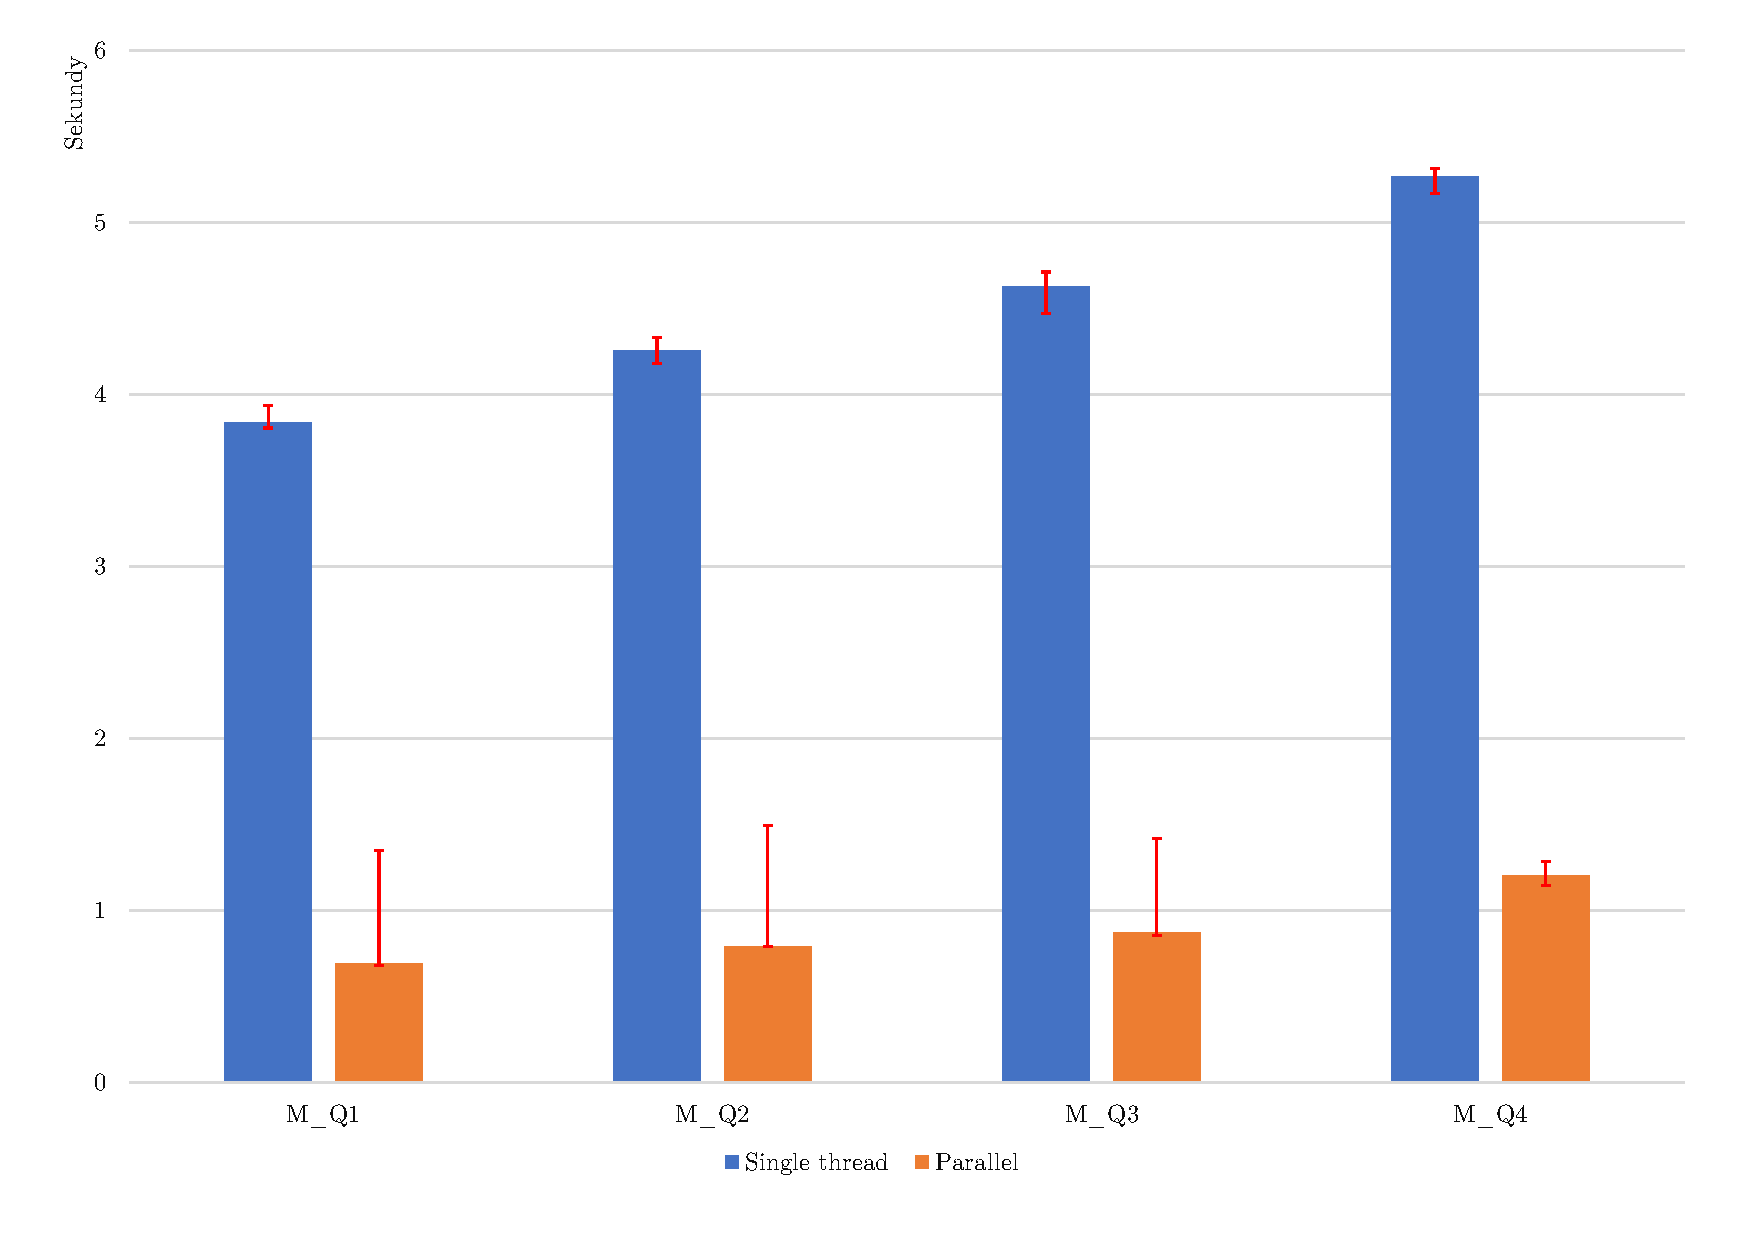
\includegraphics[width=\linewidth]{../img/amazonMatch.pdf}\centering
\caption{Doba vykonání dotazů Match pro graf Amazon0601 (sekce \ref{tab.grafBase}). Jedno vlákno vůči osmi vláknům. Počet nalezených výsledků je 32373599.}
\label{figure.amazonMatch}
\end{figure}

\begin{figure}[!htp]
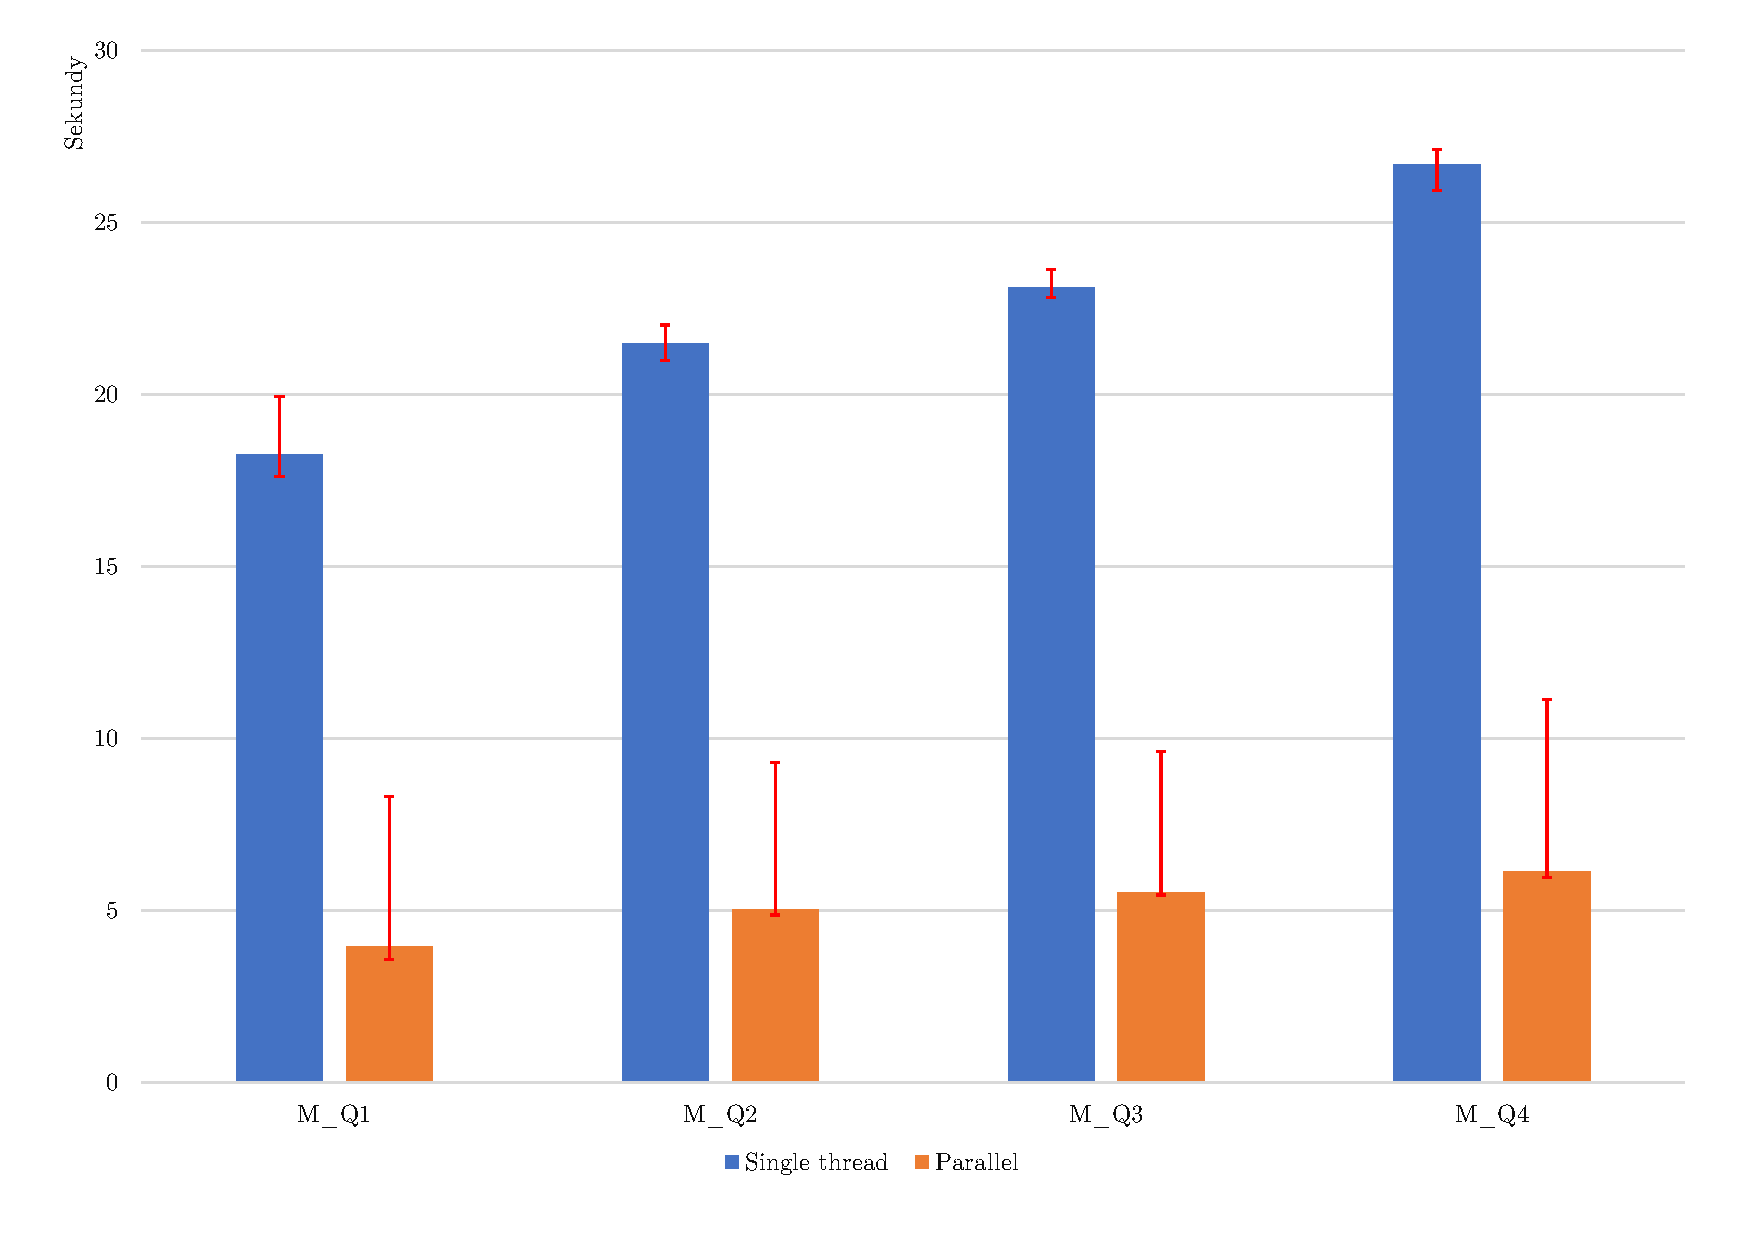
\includegraphics[width=\linewidth]{../img/webberkstanMatch.pdf}\centering
\caption{Doba vykonání dotazů Match pro graf WebBerkStan (sekce \ref{tab.grafBase}). Jedno vlákno vůči osmi vláknům. Počet nalezených výsledků je 222498869.}
\label{figure.webberkstanMatch}
\end{figure}

\begin{figure}[!htp]
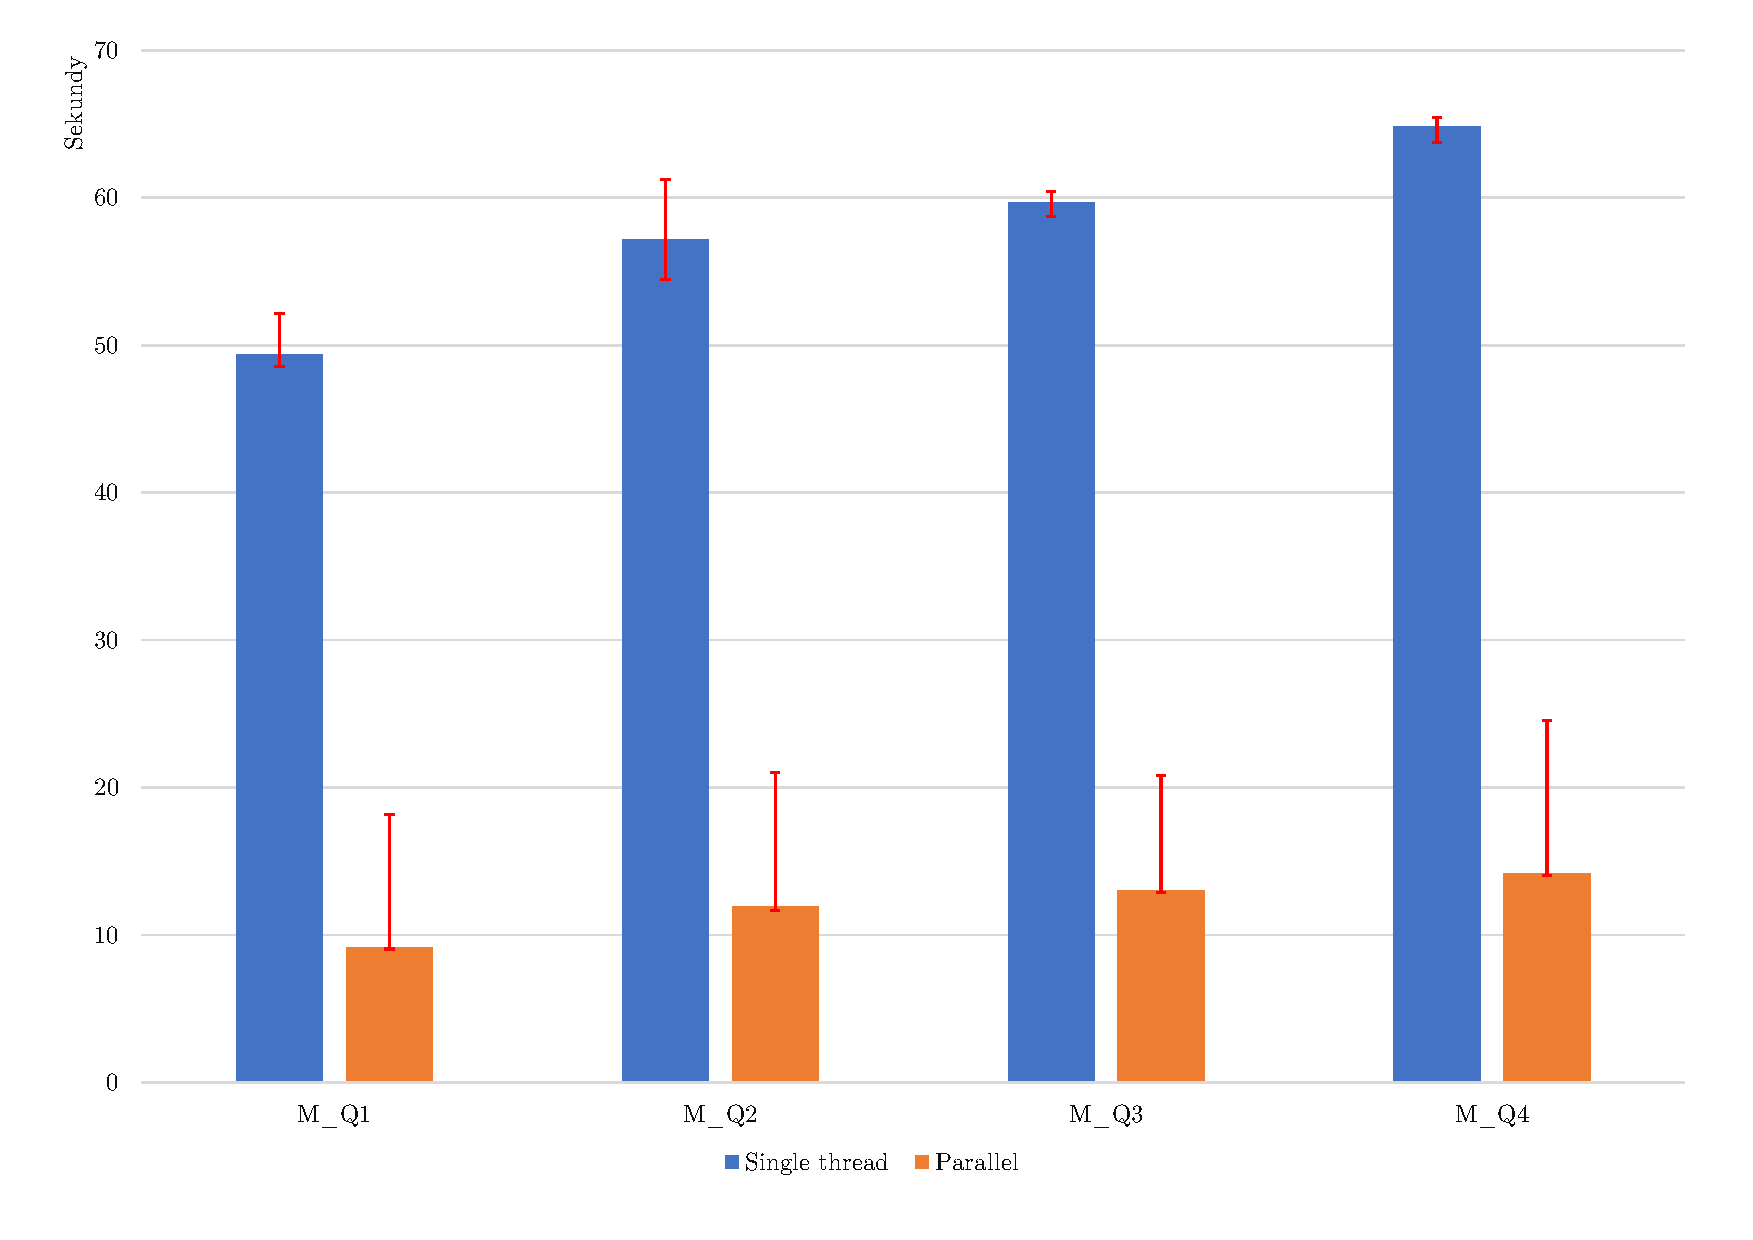
\includegraphics[width=\linewidth]{../img/skitterMatch.pdf}\centering
\caption{Doba vykonání dotazů Match pro graf As-Skitter (sekce \ref{tab.grafBase}). Jedno vlákno vůči osmi vláknům. Počet nalezených výsledků je 453674558.}
\label{figure.skitterMatch}
\end{figure}

\clearpage

Zbytek sekce věnujeme popisu obrázků \ref{figure.amazonMatch}, \ref{figure.webberkstanMatch} a \ref{figure.skitterMatch}. 
Paralelizace startovního prohledávacího vrcholu (tj. každé vlákno dostává opakovaně množství vrcholů k prohledání určené argumentem \verb+VerticesPerThread+, dokud se nevyčerpají všechny vrcholy grafu) dociluje zrychlení v rozmezí $[4,17; 5,56]$-krát pro všechny grafy.
Výsledky pro jednotlivé dotazy dopadly podle našeho očekávání. Dotaz M\_Q1 provádí pouze vyhledávání výsledků bez ukládání do tabulky a je nejrychlejší. 
Všechny ostatní dotazy dosahují zpomalení závíslé na počtu ukládaných proměnných (počet ukládaných proměnných definuje část Select), tedy čím více proměnných k uložení tím je vykonání pomalejší a to platí i pro paralelní verzi. 
Pro představu, každá proměnná (element grafu) je uložena do vlastního sloupečku, který je lokální pro vlákno (\verb+List<Element[FixedArraySize]>+). Lokalita sloupečků vede na potřebu mergování výsledků vláken. 

Nicméně, díky ukládání do polí fixní délky nastává nutnost pouze zarovnat poslední nezaplněná pole, zbytek práce mergování je jen přesunutí několika pointrů na pole. 
Tento proces je paralelizovaný pouze přes sloupečky, tedy v dotazu M\_Q2 mergování beží pouze v jednom vlákně a proto obsahuje nejvyšší skok rychlosti mezi dotazem před a dotazem po. 
Obecně vidíme, že ukládání výsledků nepřináší až tak velkou přítež na dobu vykonávání jako paměťovou, kdy všechny výsledky jsou uloženy v paměti. 
Například, všechny dotazy na grafu As-Skitter (obrázek \ref{figure.skitterMatch}), vygenerují 453674558 výsledků, což představuje na x64 platformě 3.629 GB pro jeden sloupeček.
Zmíněné poznatky použijeme při analýze experimentů pro Group/Order by.

\subsection{Order by}

Z důvodu časové a prostorové složitosti třídění na grafu As-Skitter jsme se rozhodli jej vynechat pro Order by dotazy.

Vylepšená řešení při přichozím výsledku jej uloží do tabulky (stejné tabulky jako v řešení Normal) a následně vloží index výsledku v tabulce do indexovací struktury, tj. v našem případě $(a, b)$-strom\footnote{\citet[03. (a,b)-trees]{dataLecture}}, kde $b=2a$. 
Používáme $b=256$.
V řešení ABTree se jedná o obecný $(a, b)$-strom, zatímco řešení ABTreeValueAccumulator výsledky (indexy) mající stejnou hodnotu klíčů třídění uloží do \verb+List<int>+.
Zástupce Normal řešení je Merge sort\footnote{\citet{hpcsharp}}.

Začneme řešením běžícím v jednom vlákně, tj. obrázky  \ref{figure.amazonOrderST} a \ref{figure.webberkstanOrderST}.
Můžeme si všimnout, že výsledky vypadají v rámci daných grafů konzistentně pro každý dotaz.
Ani jedno z vylepšených řešení nedokázalo porazit mód Normal, což odpovídá našim předpokladům. 
Je to protože daný strom podléhá režii za \verb+Insert+ $\Theta(\log n \cdot (a/\log a))$ (\citet[03. (a,b)-trees str. 6]{dataLecture}), kdy dochází k častému alokování nových vrcholů a překopírovávání prvků při splitu.
Nejproblematičtější část je množství tříděných výsledků, kdy počet samotných hodnot klíčů třídění je omezen počtem vrcholů v grafu (tabulka \ref{tab.grafBase}). 
Daná situace vede k opakovanému zatřizování výsledků se stejnou hodnotou a tím navyšování velikosti stromu společně s počtem porovnání na \verb+Insert+.
Celý problém jsme vyřešelili v řešení ABTreeValueAccumulator, kdy se duplicitní hodnoty ukládají do zmíněného pole a tím omezujeme velikost výsledného stromu. 
Jak vidíme na obrázcích, řešení se přibližuje rychlosti řešení Normal.

\begin{figure}[!htp]
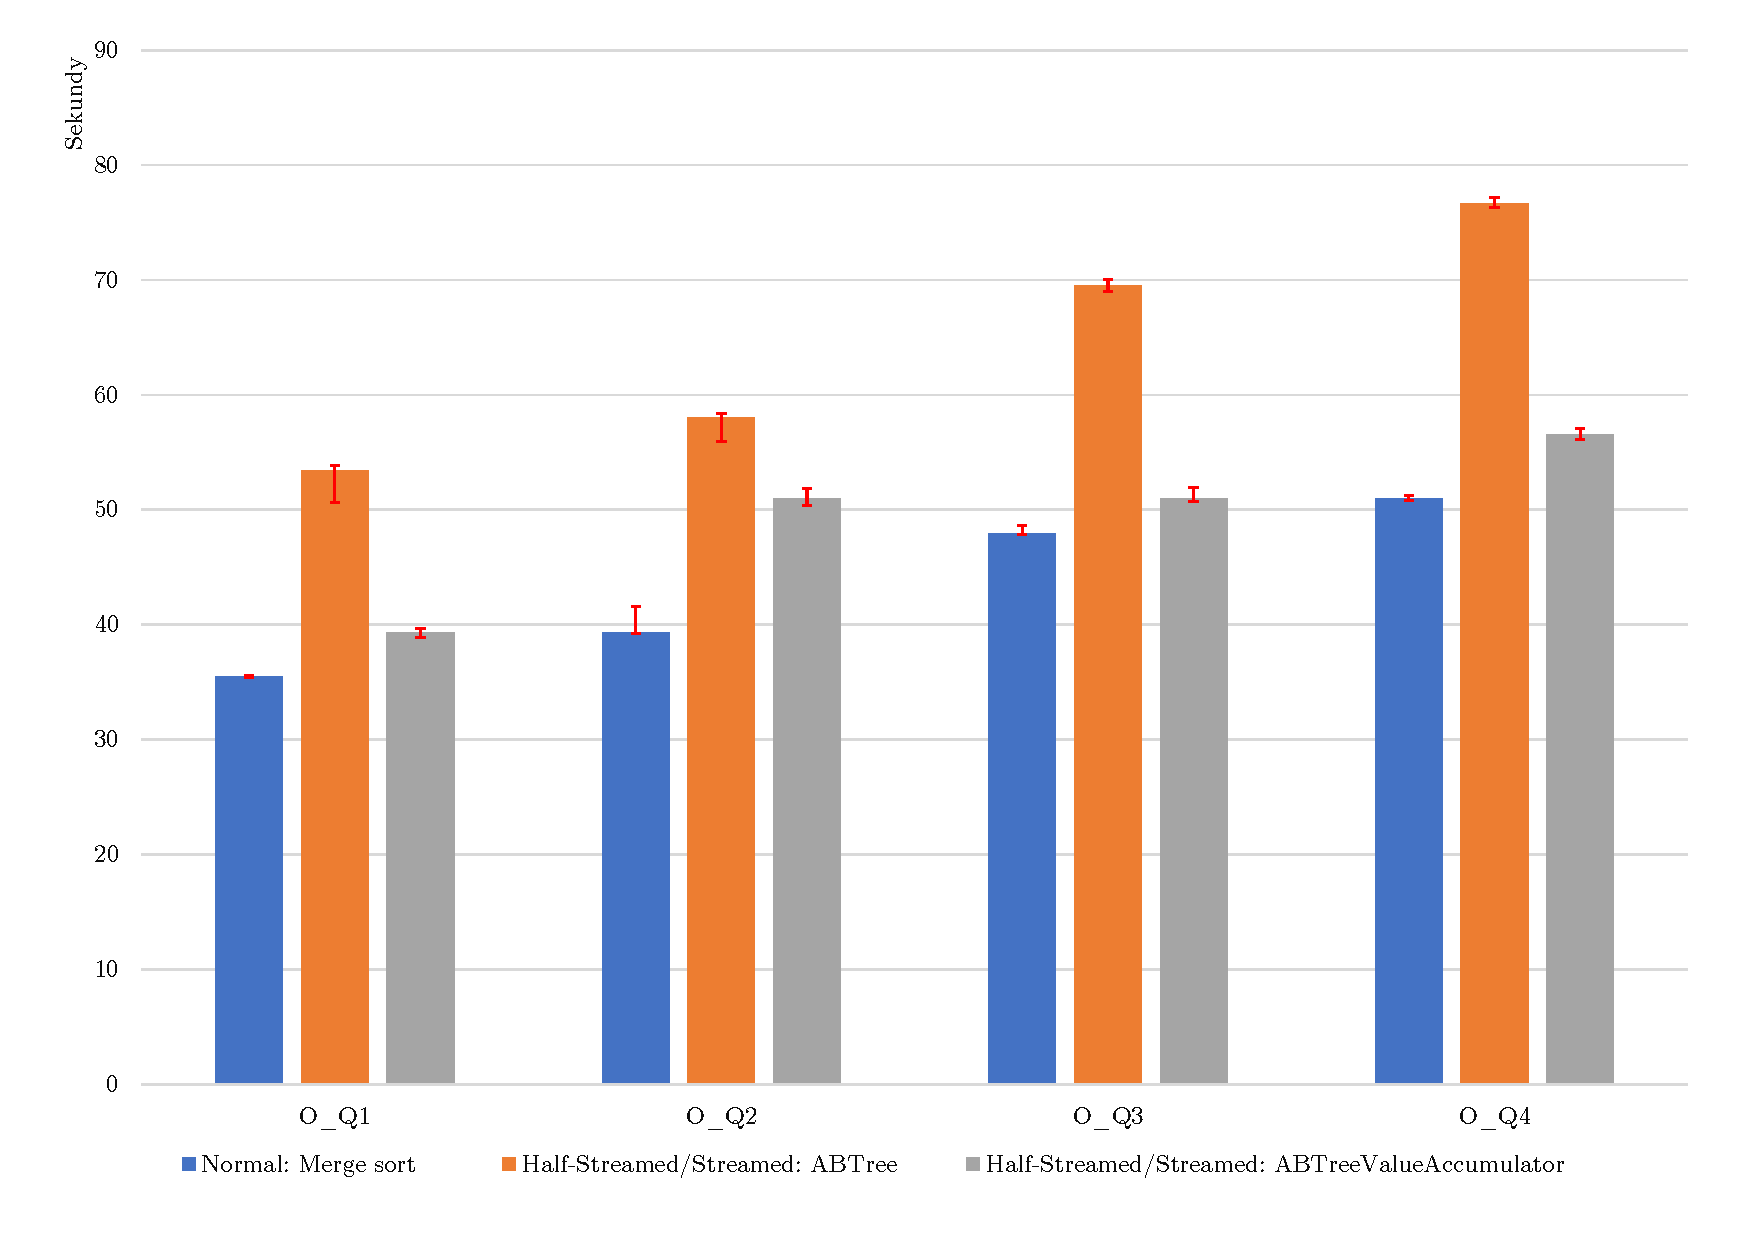
\includegraphics[width=\linewidth]{../img/amazonOrderByST.pdf}\centering
\caption{Doba vykonání dotazů Order by pro graf Amazon0601 (sekce \ref{tab.grafBase}). Běh v jednom vláknu. Počet tříděných výsledků je 32373599.}
\label{figure.amazonOrderST}
\end{figure}

\begin{figure}[!htp]
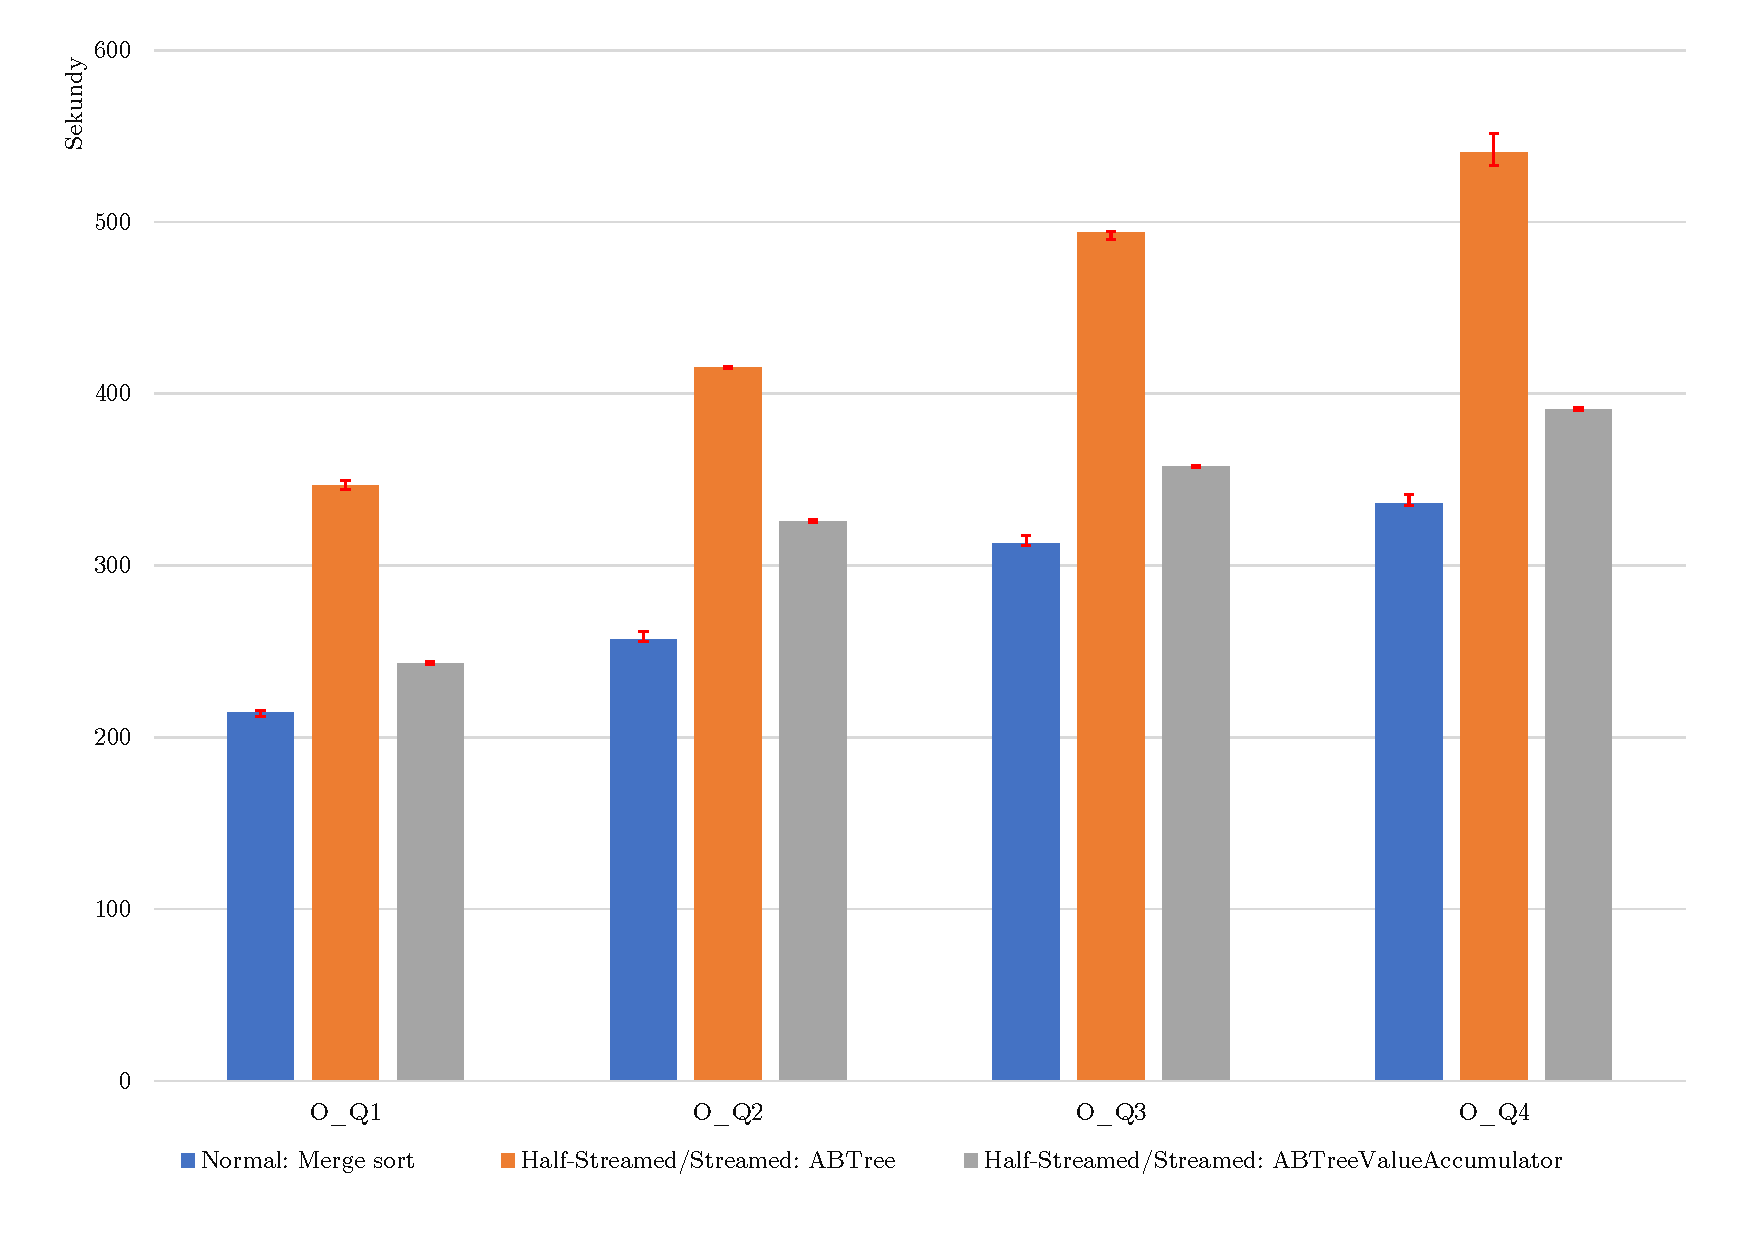
\includegraphics[width=\linewidth]{../img/webberkstanOrderByST.pdf}\centering
\caption{Doba vykonání dotazů Order by pro graf WebBerkStan (sekce \ref{tab.grafBase}). Běh v jednom vláknu. Počet tříděných výsledků je 222498869.}
\label{figure.webberkstanOrderST}
\end{figure}

\clearpage


Problém by nastal, pokud by množství hodnot odpovídalo počtu nalezených výsledků. 
V tomto případě bychom vytvářeli zbytečný overhead za režii pole.
Dle našich předpokladů se ukázalo, že třídění podle \verb+ID+ (O\_Q1 a O\_Q2) vůči Properties (O\_Q3 a O\_Q4) vede ke znatelnému overheadu.
Je to způsobeno nutným přístupem k databázi, při kterém se ověřuje, jestli daná vlastnost existuje na daném elementu a následném čtení hodnoty ze struktury obsahující ji.

Paralelní zpracování aplikuje použité verze $(a, b)$-stromů ze zpracování pro jedno vlákno. 
Half-Streamed řešení obsahuje lokální tabulku a indexační strom pro každé běžící vlákno. 
Po dokončení vyhledávání se obsahy stromů překopírují do pole a dojde k paralelnímu 2-way merge používající stejnou funkci jako paralelní Merge sort. 
Streamed řešení rozdělí rozsah prvního třídícího klíče do přihrádek rovnoměrné velikosti. 
Při příchozím výsledku se získá hodnota prvního klíče třídění a určí se jeho přihrádka. 
Počet přihrádek je heuristicky zvolen jako $m=t^2$, kde $t=\#vláken$. 
Samotná přihrádka obsahuje opět tabulku a indexační strom přistupné pomocí zámku. 
Při porovnávání je nutné mít na paměti, že lokálně bežící části používájí cachování popsané v sekci (TODO).  

Nyní budeme prezetovat výsledky paralelizace (obrázky \ref{figure.amazonOrderPar} a \ref{figure.webberkstanOrderPar}).
Pro dotazy O\_Q1 a O\_Q2 vidíme u Streamed řešení mnohonásobný rozdíl vůči ostatním řešením, protože přihrádky jsou rozděleny na základě rozsahu typu klíče (např. pro O\_Q3 $[$\verb+Int32.MinValue+; \verb+Int32.MaxValue+$]$).
Avšak, hodnoty třídění spadají do rozsahu \verb+ID+ vrcholů grafu, což představuje rozsah $\approx [0; \#vrcholů]$. 
Hodnota třídění spadá vždy do jedné přihrádky a výsledná doba je rovna době single thread řešení s overheadem za přistupovaný zámek.
Pro O\_Q1 je to zpomalení o $[20,51; 21]$\% a pro O\_Q2 $[17,64; 18,9]$\%.
U dotazů O\_Q3 a O\_Q4 je tříděno pomocí hodnot vygenerovaných náhodně spadající do celého rozsahu typu klíče a zde Streamed řešení předčilo všechna ostatní. 
Pro budoucí rozšíření by bylo nutné zvážit vytvoření statistik rozsahů jednotlivých Properties, aby bylo možné lépe vytvořit rozdělení přihrádek.

Half-Streamed řešení se přibližuje Normal řešení v prvních dvou dotazech a překonává jej ve třetím i čtvrtém dotazu pro řešení používající ABTreeValueAccumulator.
U třetího a čtvrtého dotazu se porovnává pomocí Properties. V single thread zpracovávání jsme viděli overhead za dané porovnání.
V druhém kroku u daného Half-Streamed řešení dochází k mergování pouze akumulovaných skupin, což rapidně sníží počet porovnávání při mergi a odtud výhoda oproti Normal Merge sort řešení. 
To samé platí u Streamed řešení, protože počáteční rozhašování způsobí vkládání do mnohonásobně menší skupiny výsledků. 
Celá situace je navíc umocněna zmíněným cachovaním porovnávaných hodnot. 

Zajímavý výsledek testování je rozsah zrychlení vylepšených módů (tabulka \ref{tab.OrderByZrychleni}), který jsme neočekávali. 
Zrychlení Merge sortu zaostavá. Maximální zrychlení u ostatních řešení je až pětinásobné. 
Implementace paralelního Merge sortu funguje na principu postupného rekurzivního rozdělování, při kterém se vytváří nové \verb+Tasks+ pro \verb+ThreadPool+.
U vylepšených řešení běži jedna metoda pro každé vlákno po dobu celého zpracování. Jestli se jedná o hlavní důvod poznatku by vyžadovalo dalšího testování. 

Jako důsledek testování můžeme konstatovat, že třídění v průběhu vyhledávání nepřináší předpokládané výhody.
Zrychlení nastává pouze u paralelizace řešení při dostatečně náhodném rozložení dat třídění, pokud samotná porovnání jsou drahá.

\begin{figure}[!htp]
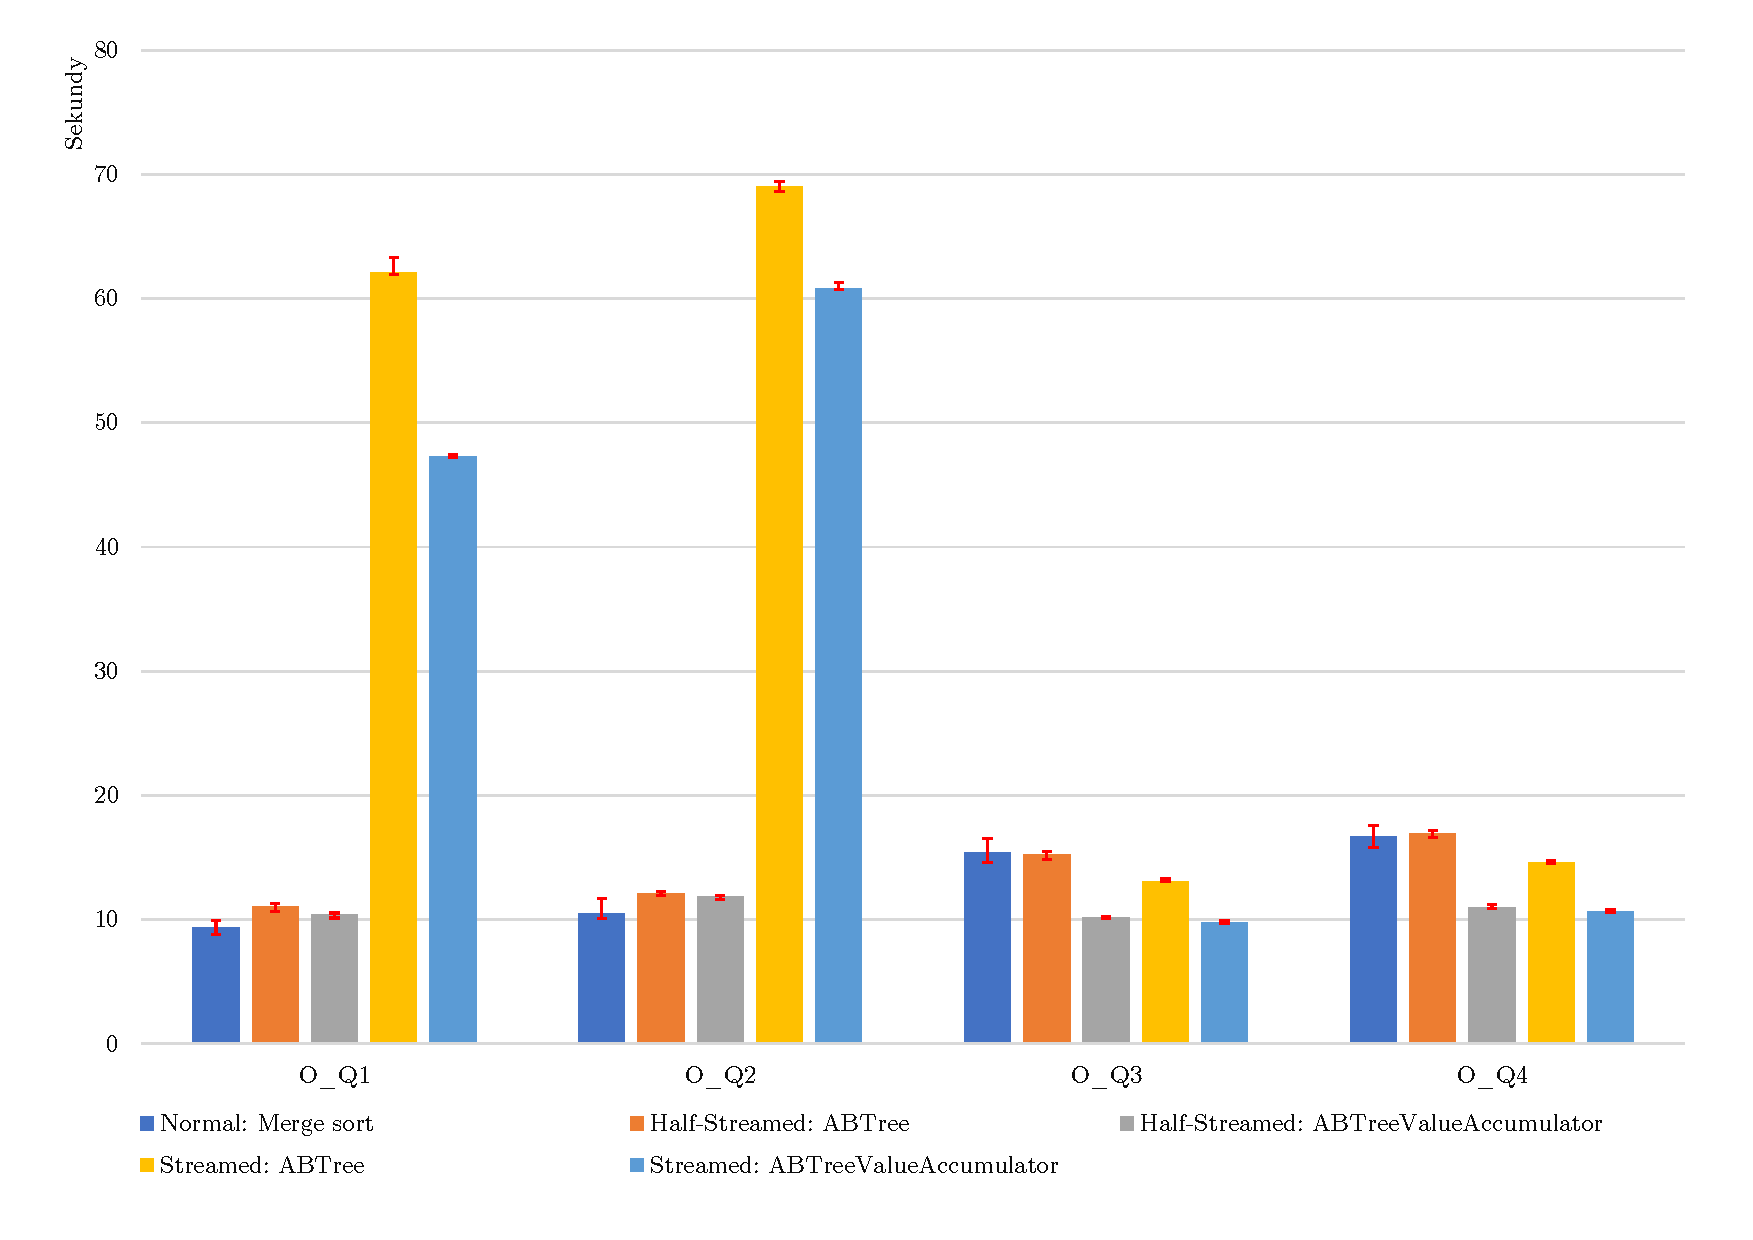
\includegraphics[width=\linewidth]{../img/amazonOrderByPar.pdf}\centering
\caption{Doba vykonání dotazů Order by pro graf Amazon0601 (sekce \ref{tab.grafBase}).  Běh osmi vláken. Počet tříděných výsledků je 222498869.}
\label{figure.amazonOrderPar}
\end{figure}

\begin{figure}[!htp]
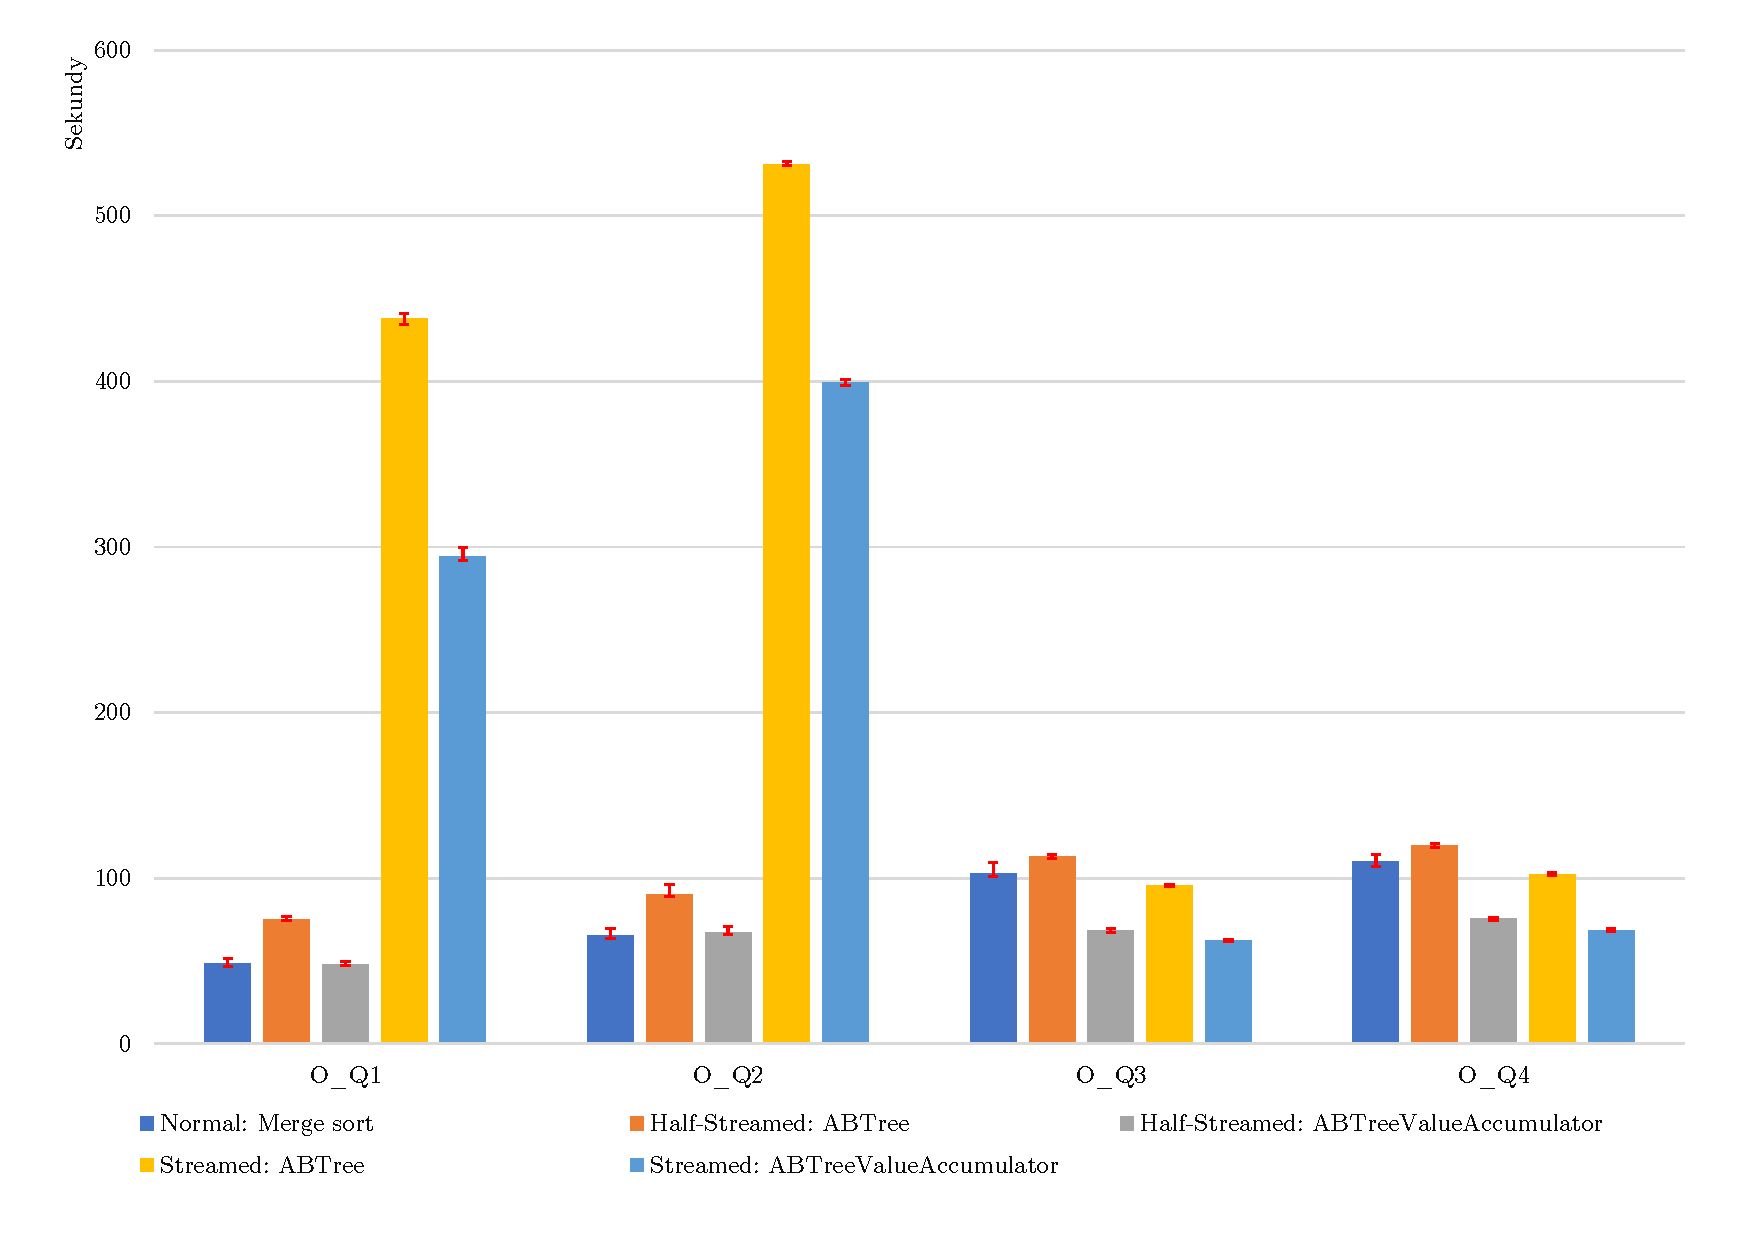
\includegraphics[width=\linewidth]{../img/webberkstanOrderByPar.pdf}\centering
\caption{Doba vykonání dotazů Order by pro graf WebBerkStan (sekce \ref{tab.grafBase}).  Běh osmi vláken. Počet tříděných výsledků je 222498869.}
\label{figure.webberkstanOrderPar}
\end{figure}

\clearpage

\begin{table}[!htb]
\centering
\begin{tabular}{lr}
\toprule
\mc{} & \mc{\textbf{Zrychlení}} \\
\midrule
Merge sort &  $[3,33; 4,42]$-krát \\
Half-Streamed: ABTree & $[4,36; 4,81]$-krát  \\
Half-Streamed: ABTreeValueAccumulator & $[3,76; 5,18]$-krát \\
Streamed: ABTree & $[0,78; 5,3]$-krát  \\
Streamed: ABTreeValueAccumulator & $[0,81; 5,72]$-krát \\
\bottomrule
\end{tabular}

\caption{Rozsah zrychlení paralelizovaných řešení pomocí osmi vláken v ramci grafů pro dotazy Order by.}
\label{tab.OrderByZrychleni}
\end{table}

\subsection{Group by}

Analýzu výsledků dotazu G\_Q1 uvádíme samostatně, protože testuje pouze agregační funkce a nikoliv seskupování.
Po levé straně je běh v jednom vlákně a na pravé straně běh osmi vláken.

\begin{figure}[!htp]
    \centering
    \begin{minipage}{0.45\textwidth}
        \centering
        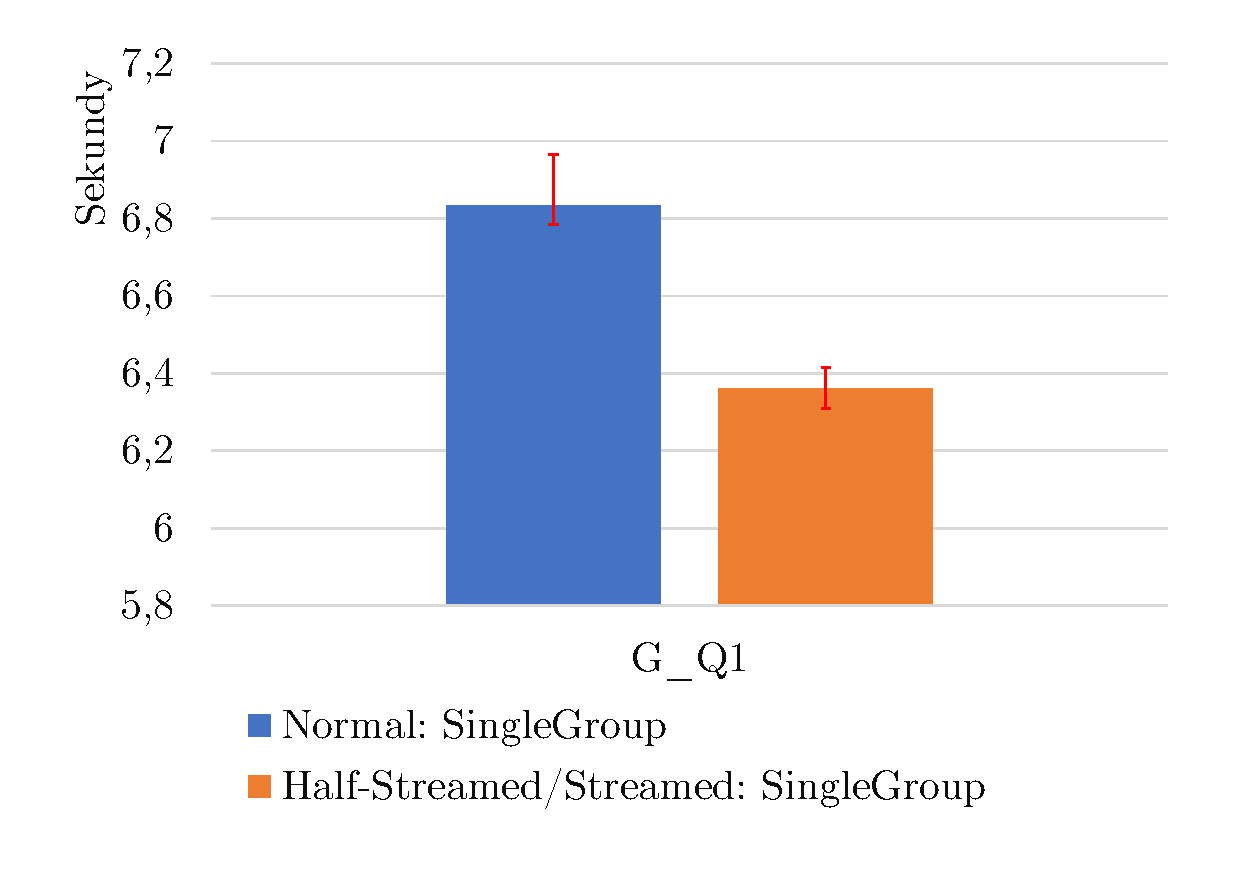
\includegraphics[width=0.9\textwidth]{../img/amazonGroupByQ1ST.pdf} % first figure itself
        \caption{Doba vykonání dotazu G\_Q1 pro graf Amazon0601 (sekce \ref{tab.grafBase}). Běh v jednom vláknu. Počet seskupovaných výsledků je 32373599.}
        \label{figure.amazonGQ1ST}
    \end{minipage}\hfill
    \begin{minipage}{0.45\textwidth}
        \centering
        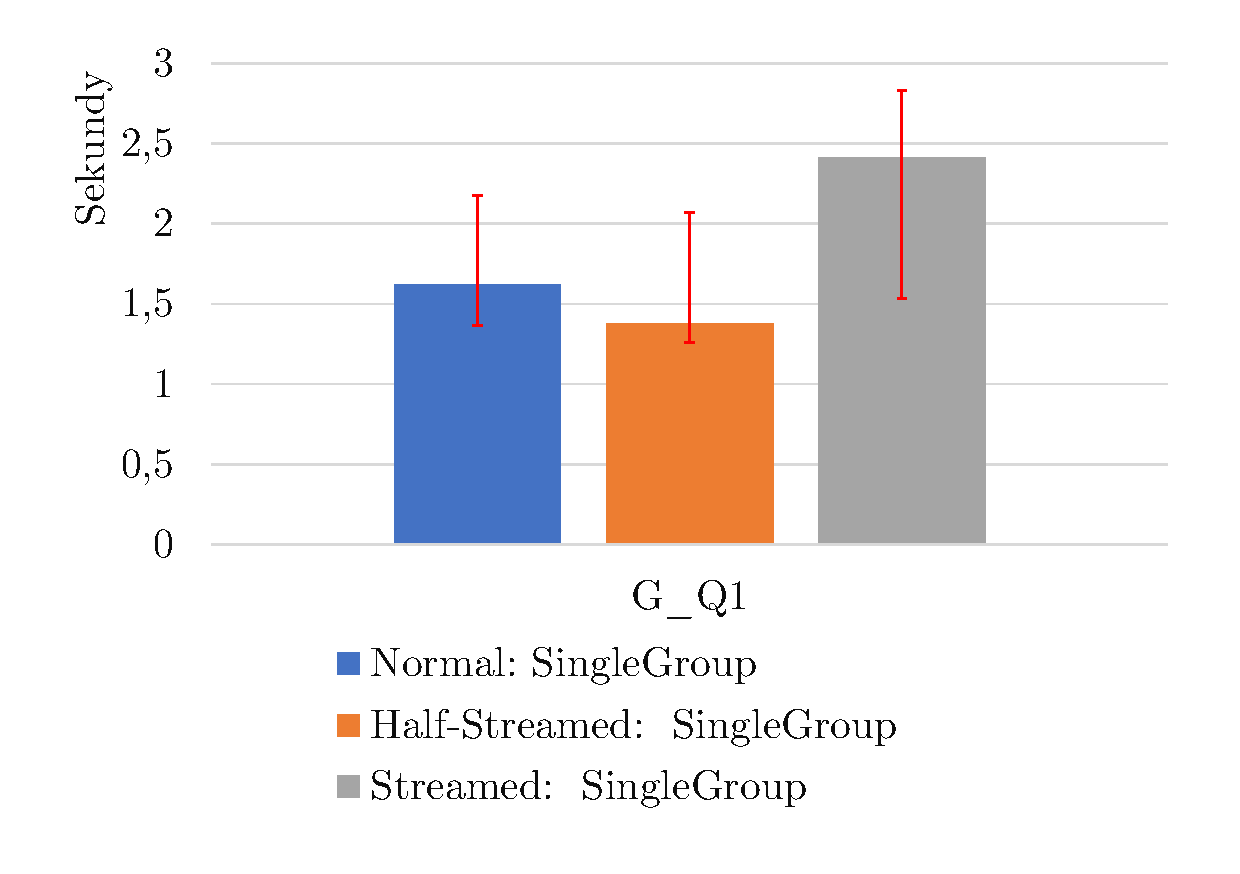
\includegraphics[width=0.9\textwidth]{../img/amazonGroupByQ1Par.pdf} % second figure itself
        \caption{Doba vykonání dotazu G\_Q1 pro graf Amazon0601 (sekce \ref{tab.grafBase}). Běh osmi vláken. Počet seskupovaných výsledků je 32373599.}
        \label{figure.amazonGQ1Par}
    \end{minipage}
\end{figure}

\begin{figure}[!htp]
    \centering
    \begin{minipage}{0.45\textwidth}
        \centering
        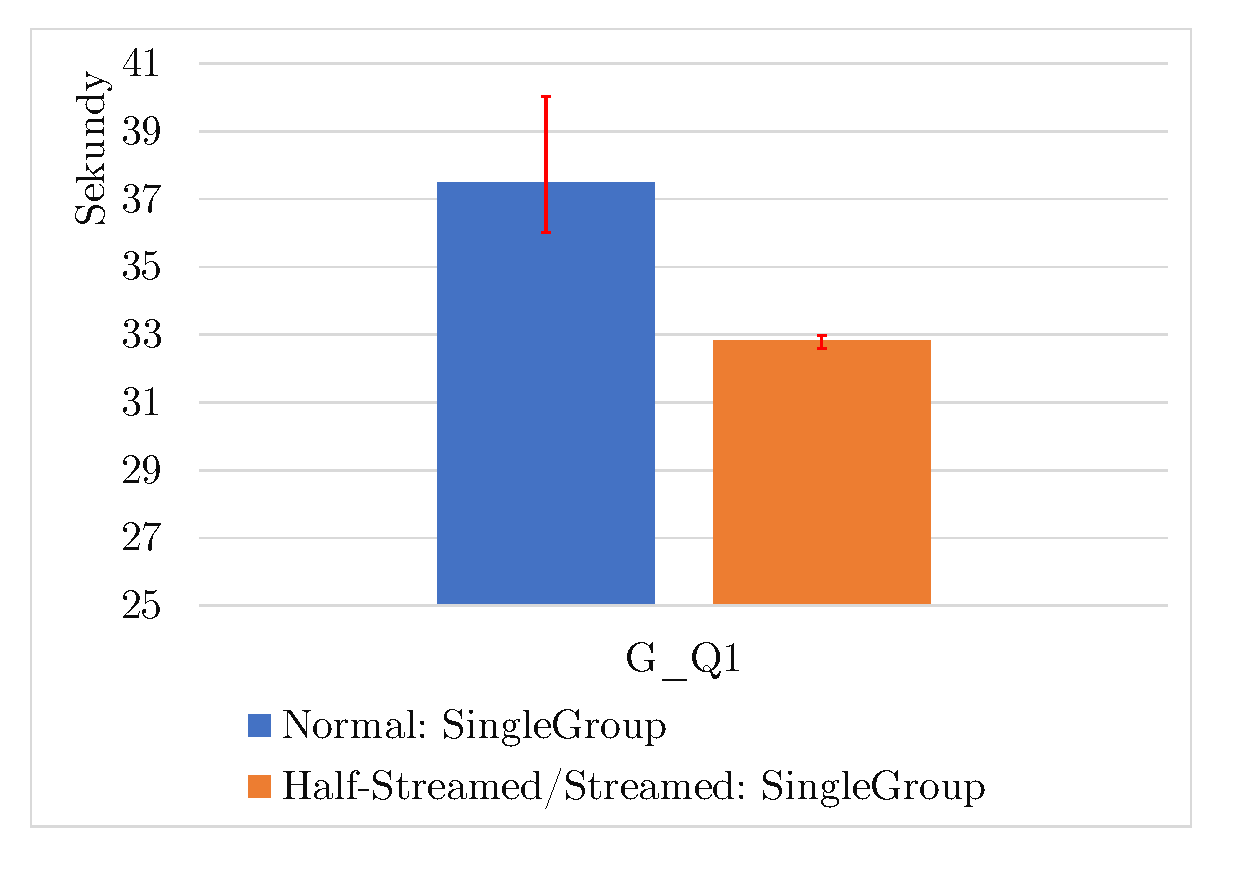
\includegraphics[width=0.9\textwidth]{../img/webberkstanGroupByQ1ST.pdf} % first figure itself
        \caption{Doba vykonání dotazu G\_Q1 pro graf WebBerkStan (sekce \ref{tab.grafBase}). Běh v jednom vláknu. Počet seskupovaných výsledků je 222498869.}
        \label{figure.webberkstanGQ1ST}
    \end{minipage}\hfill
    \begin{minipage}{0.45\textwidth}
        \centering
        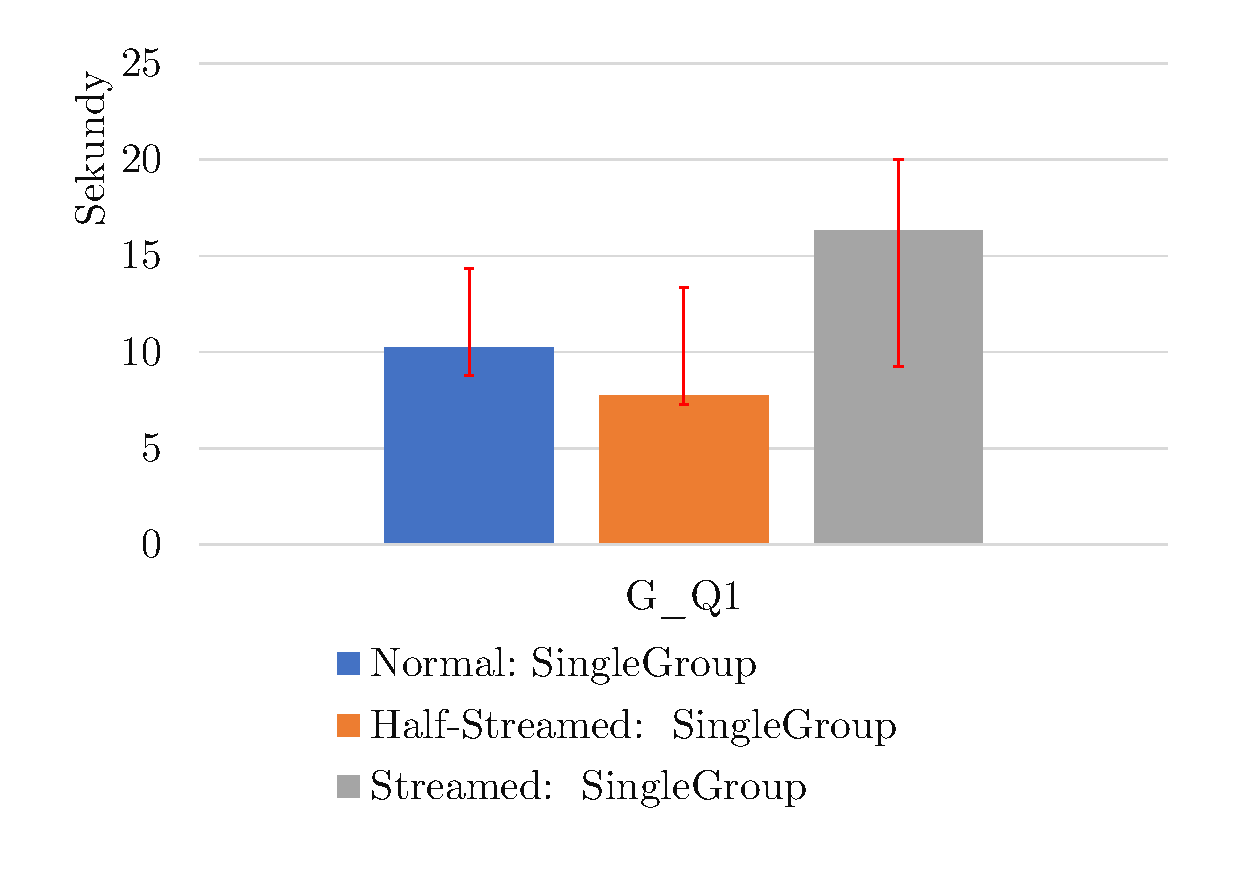
\includegraphics[width=0.9\textwidth]{../img/webberkstanGroupByQ1Par.pdf} % second figure itself
        \caption{Doba vykonání dotazu G\_Q1 pro graf WebBerkStan (sekce \ref{tab.grafBase}). Běh osmi vláken. Počet seskupovaných výsledků je 222498869.}
        \label{figure.webberkstanGQ1Par}
    \end{minipage}
\end{figure}

\clearpage

\begin{figure}[!htp]
    \centering
    \begin{minipage}{0.45\textwidth}
        \centering
        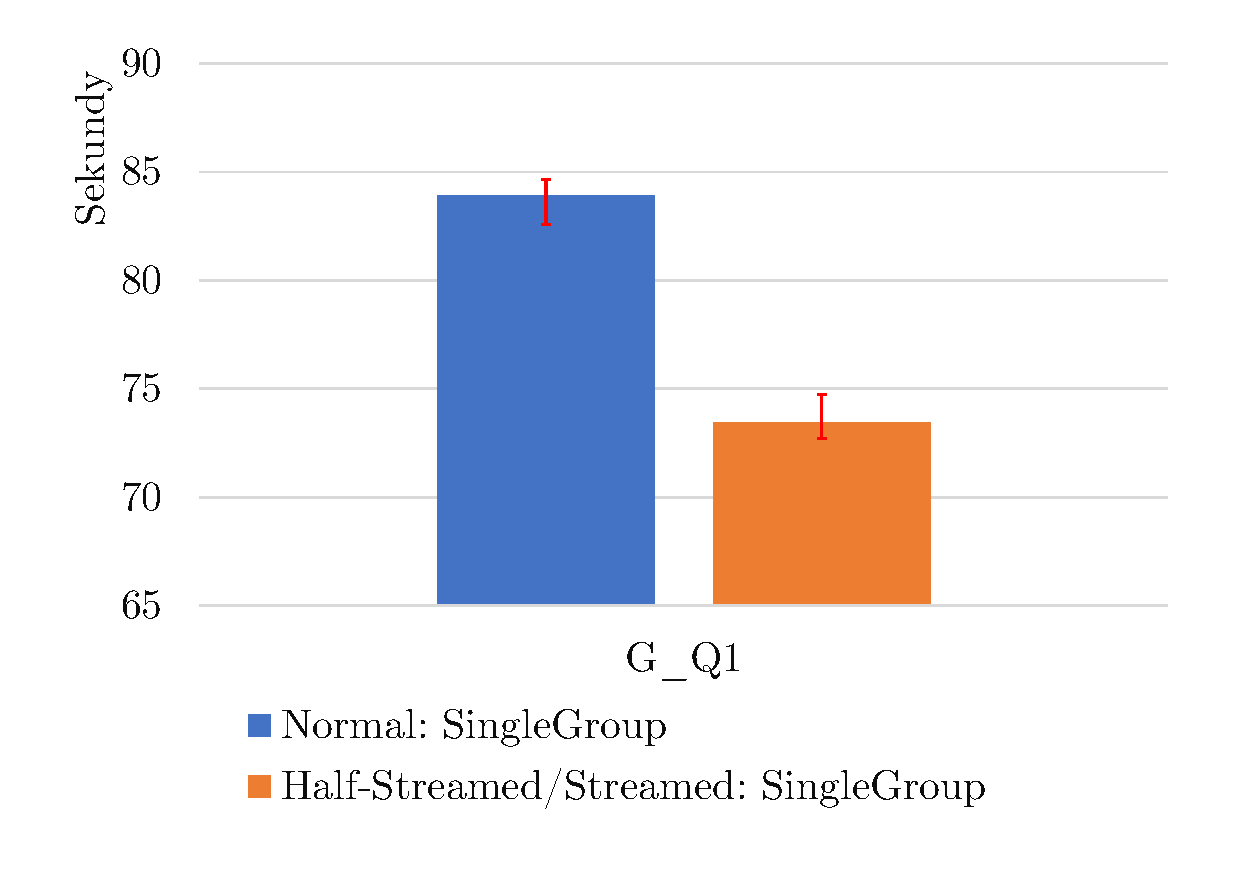
\includegraphics[width=0.9\textwidth]{../img/skitterGroupByQ1ST.pdf} % first figure itself
        \caption{Doba vykonání dotazu G\_Q1 pro graf As-Skitter (sekce \ref{tab.grafBase}). Běh v jednom vláknu. Počet seskupovaných výsledků je 453674558.}
        \label{figure.skitterGQ1ST}
    \end{minipage}\hfill
    \begin{minipage}{0.45\textwidth}
        \centering
        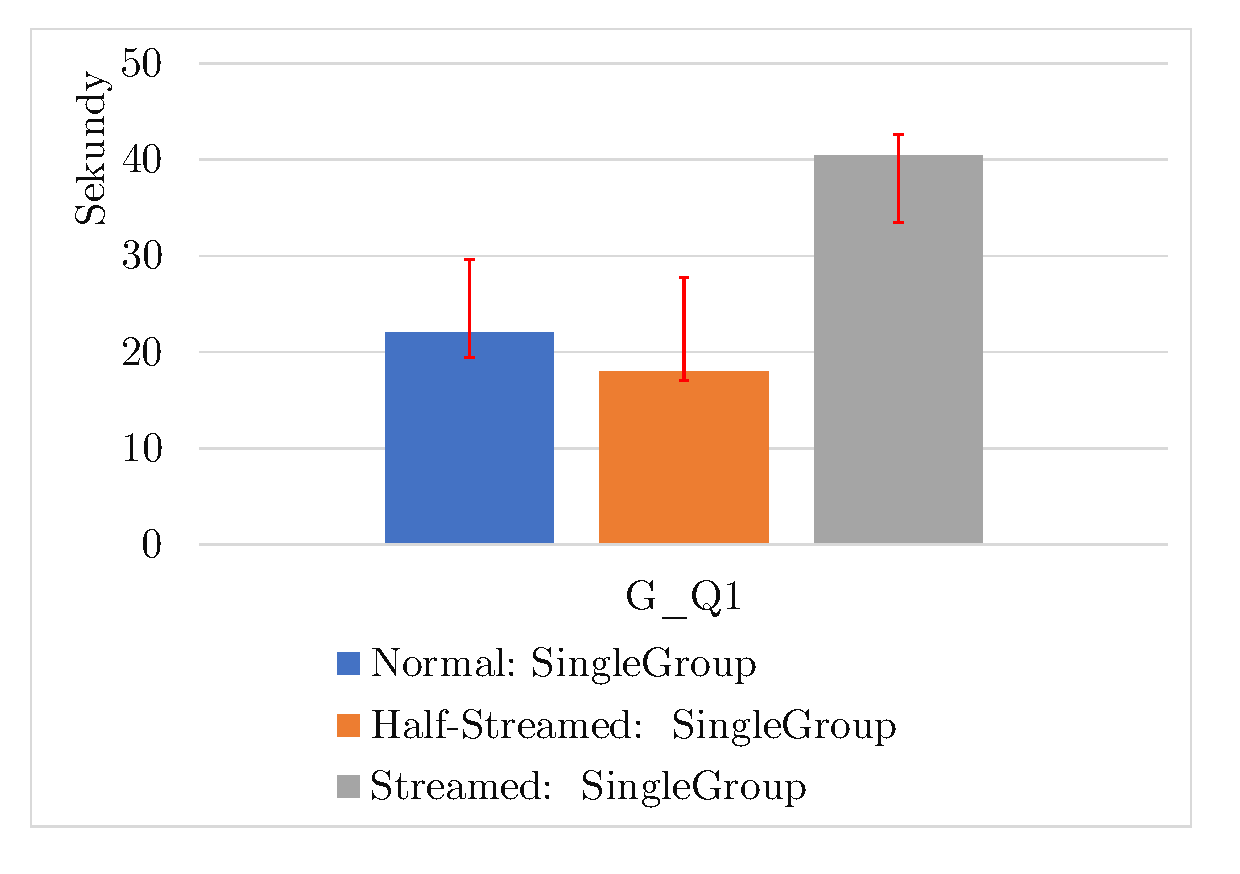
\includegraphics[width=0.9\textwidth]{../img/skitterGroupByQ1Par.pdf} % second figure itself
        \caption{Doba vykonání dotazu G\_Q1 pro graf As-Skitter (sekce \ref{tab.grafBase}). Běh osmi vláken. Počet seskupovaných výsledků je 453674558.}
        \label{figure.skitterGQ1Par}
    \end{minipage}
\end{figure}

Na obrázcích \ref{figure.amazonGQ1ST} až \ref{figure.skitterGQ1Par} lze vidět značnou konzistenci mezi výsledky testování při nárustu počtu výsledků vyhledávání.
Half-Streamed a Streamed řešení zde neukládá výsledky vyhledávání do tabulky, ale pouze na aktuální výsledek aplikuje agregační funkce a následně jej zahodí.
To způsobuje značnou výhodu oproti Normal řešení, které drží všechny výsledky v paměti.
Použijeme-li poznatky z sekce \ref{matchResults} o zpomalení způsobeném ukládáním výsledků do tabulky zjistíme (v našem případě jedné proměnné), že rozdíl mezi Normal a Half-Streamed řešením se pohybuje právě v rozsahu onoho zpomalení.
To platí pro běh jednoho vlákna i běhu osmi vláken. 
Problem představuje paralelní Streamed řešení, jelikož k jednomu výsledku přistupuje osm vláken najednou, což způsobuje značné zpomalení kvůli nutné synchronizaci při výpočtu funkcí \verb+min+ a \verb+avg+. 
Zrychlení je zde pouze v rozsahu $[1,81; 2,64]$-krát, zatímco u zbylých řešení je $[3,67; 4,61]$-krát.

Než postoupíme dál připomeneme hlavní rozdíly řešení a značení u zobrazených grafů. 
Každé řešení používá k Group by mapu (\verb+Dictionary<key, value>+).
Normal řešení ukládá všechny výsledky vyhledávání vzoru do tabulky a po dokončení vykoná Group by. 
Half-Streamed řešení vykonává Group by v průběhu hledání a ukládá do tabulky pouze výsledky, pro které ještě neexistuje skupina v použité mapě.
Pro zmíněná řešení se jako \verb+key+ používá index do tabulky a skrze něj se následně výpočtou hodnoty klíče.
Streamed řešení nepoužívá tabulku, ale hodnoty klíče ukládá rovnou do mapy. 
Objevující se značení Bucket a List určuje způsob ukládání výsledků agregačních funkcí (\verb+min+, \verb+avg+...) jako \verb+value+ záznam v mapě:

\begin{code}
Bucket:
Dictionary<key, BucketResult[]> map; // Used map.
class BucketResult {}
class BucketResult<T>: BucketResult { T value; }

List:
Dictionary<key, tableIndex> map; // Used map.
ListResults aggResults; // Agg. func. values of a group 
                        // are accessed via tableIndex.
class ListResults { ListHolder[] holders; }
class ListHolder {}
class ListHolder<T> : ListHolder { List<T> values }
\end{code}

\begin{figure}[!htp]
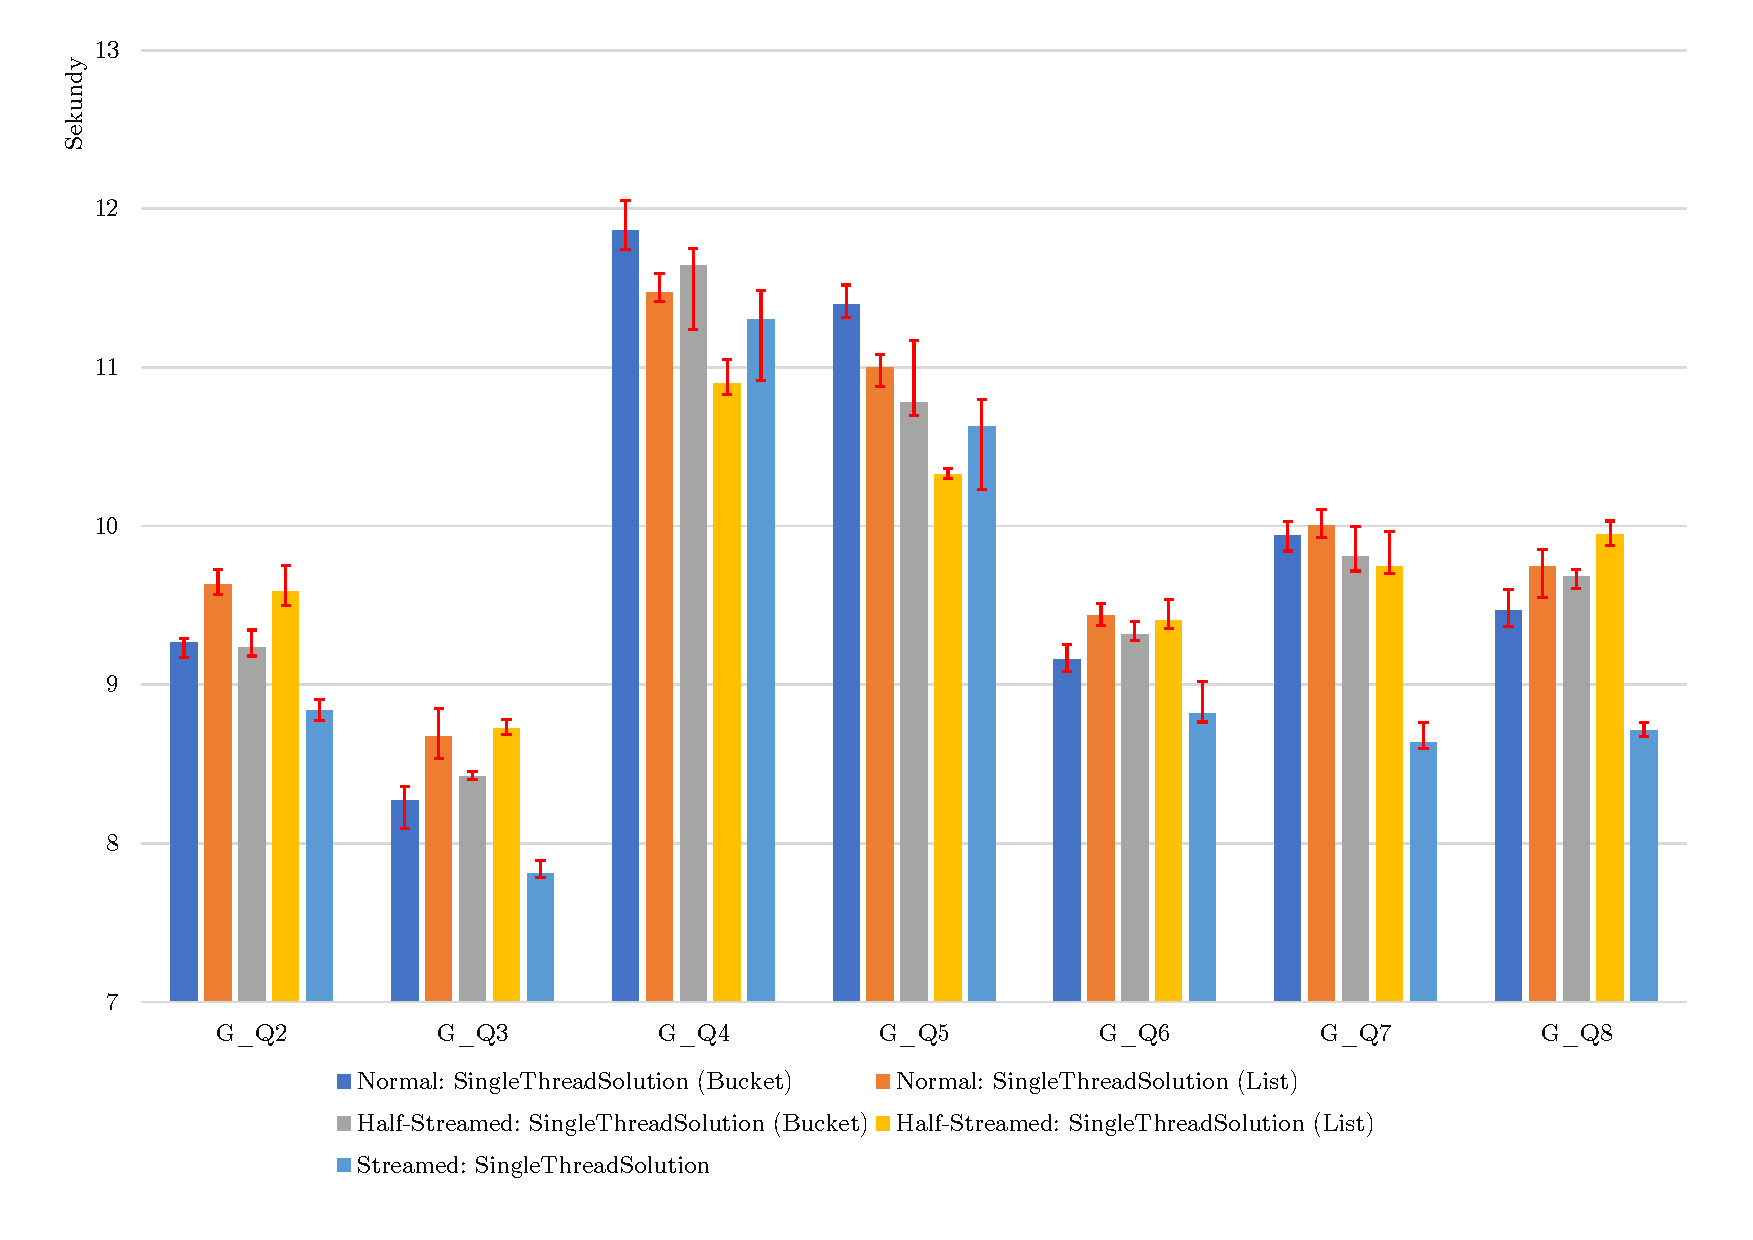
\includegraphics[width=\linewidth]{../img/amazonGroupByST.pdf}\centering
\caption{Doba vykonání dotazů Group by pro graf Amazon0601 (sekce \ref{tab.grafBase}). Běh v jednom vláknu. Počet seskupovaných výsledků je 32373599.}
\label{figure.amazonGroupByST}
\end{figure}
\begin{figure}[!htp]
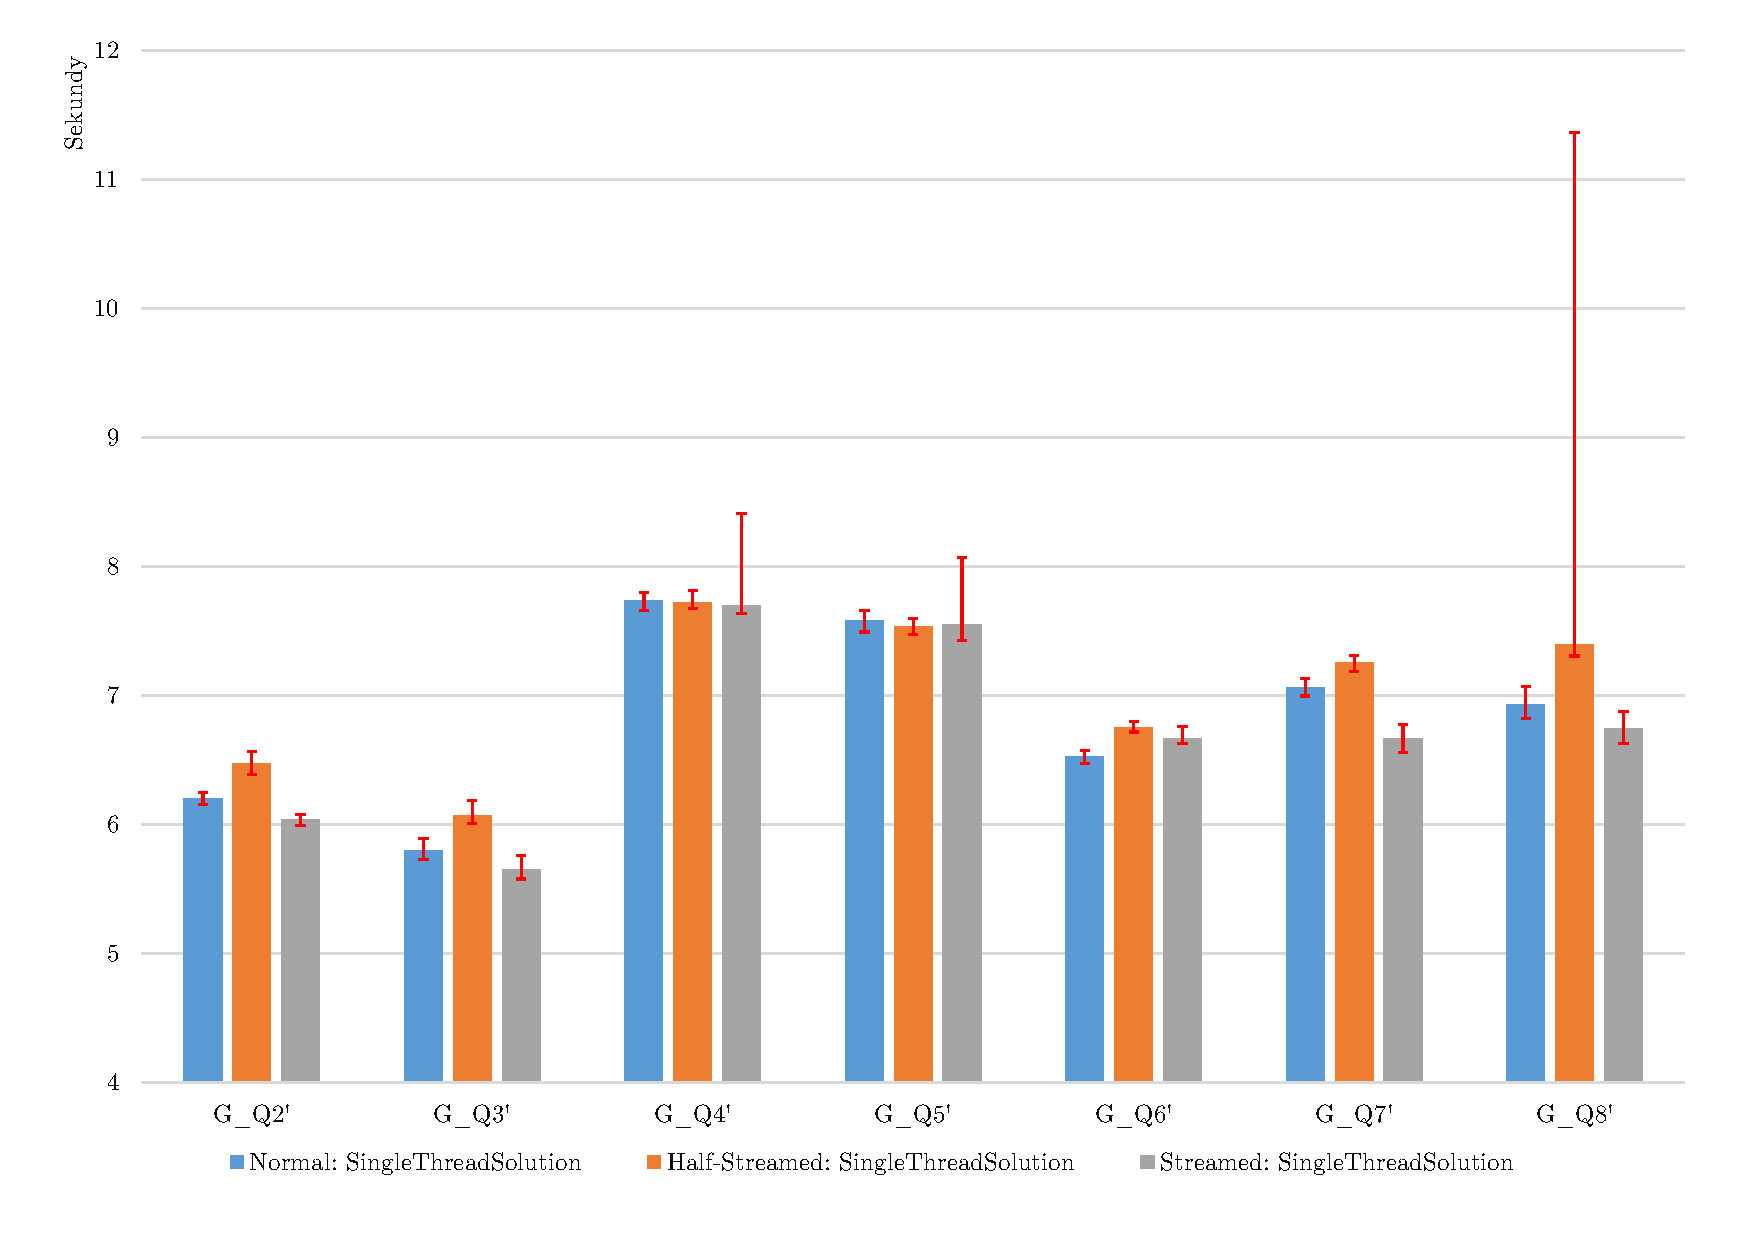
\includegraphics[width=\linewidth]{../img/amazonGroupBySTNoAgg.pdf}\centering
\caption{Doba vykonání dotazů Group by bez agr. funkcí pro graf Amazon0601 (sekce \ref{tab.grafBase}). Běh v jednom vláknu. Počet seskupovaných výsledků je 32373599.}
\label{figure.amazonGroupBySTNoAgg}
\end{figure}


\begin{figure}[!htp]
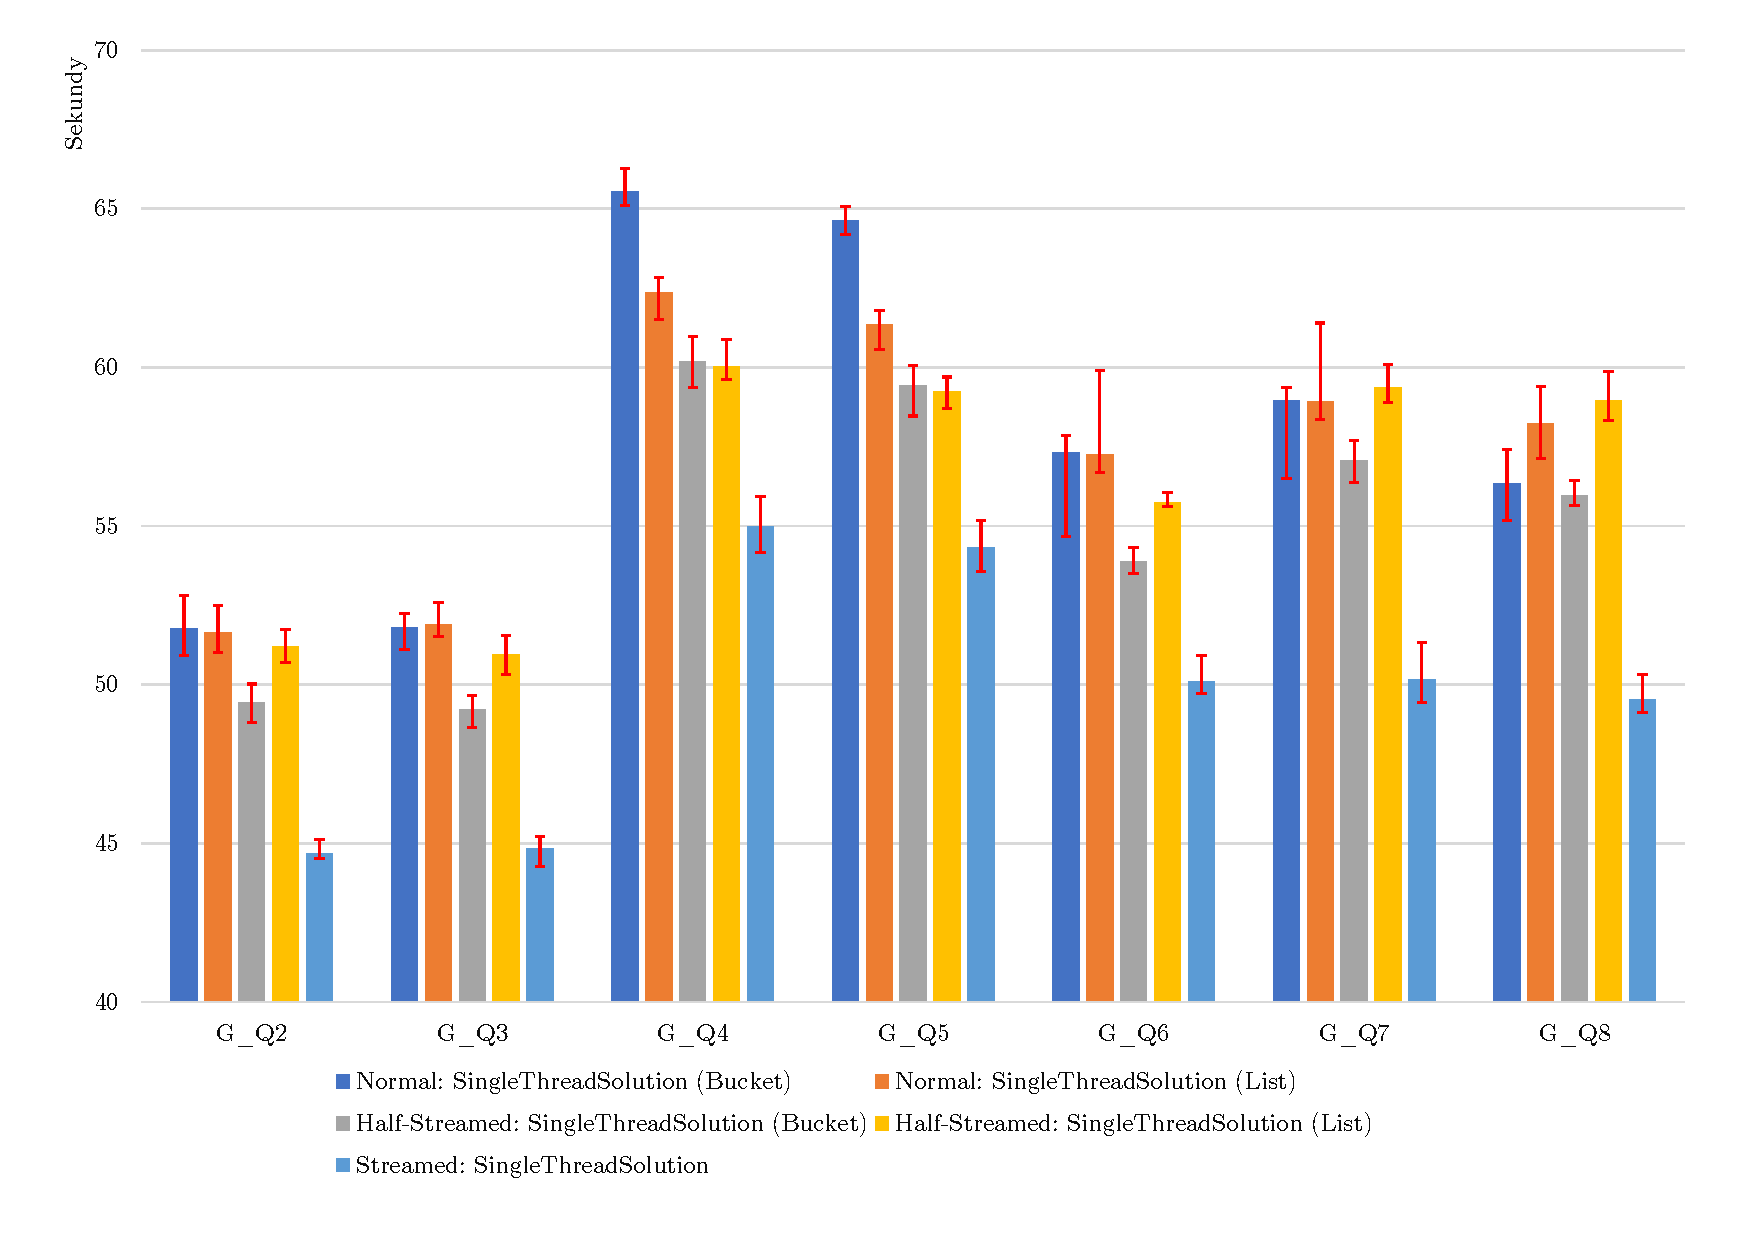
\includegraphics[width=\linewidth]{../img/webberkstanGroupByST.pdf}\centering
\caption{Doba vykonání dotazů Group by pro graf WebBerkStan (sekce \ref{tab.grafBase}). Běh v jednom vláknu. Počet seskupovaných výsledků je 222498869.}
\label{figure.webberkstanGroupByST}
\end{figure}
\begin{figure}[!htp]
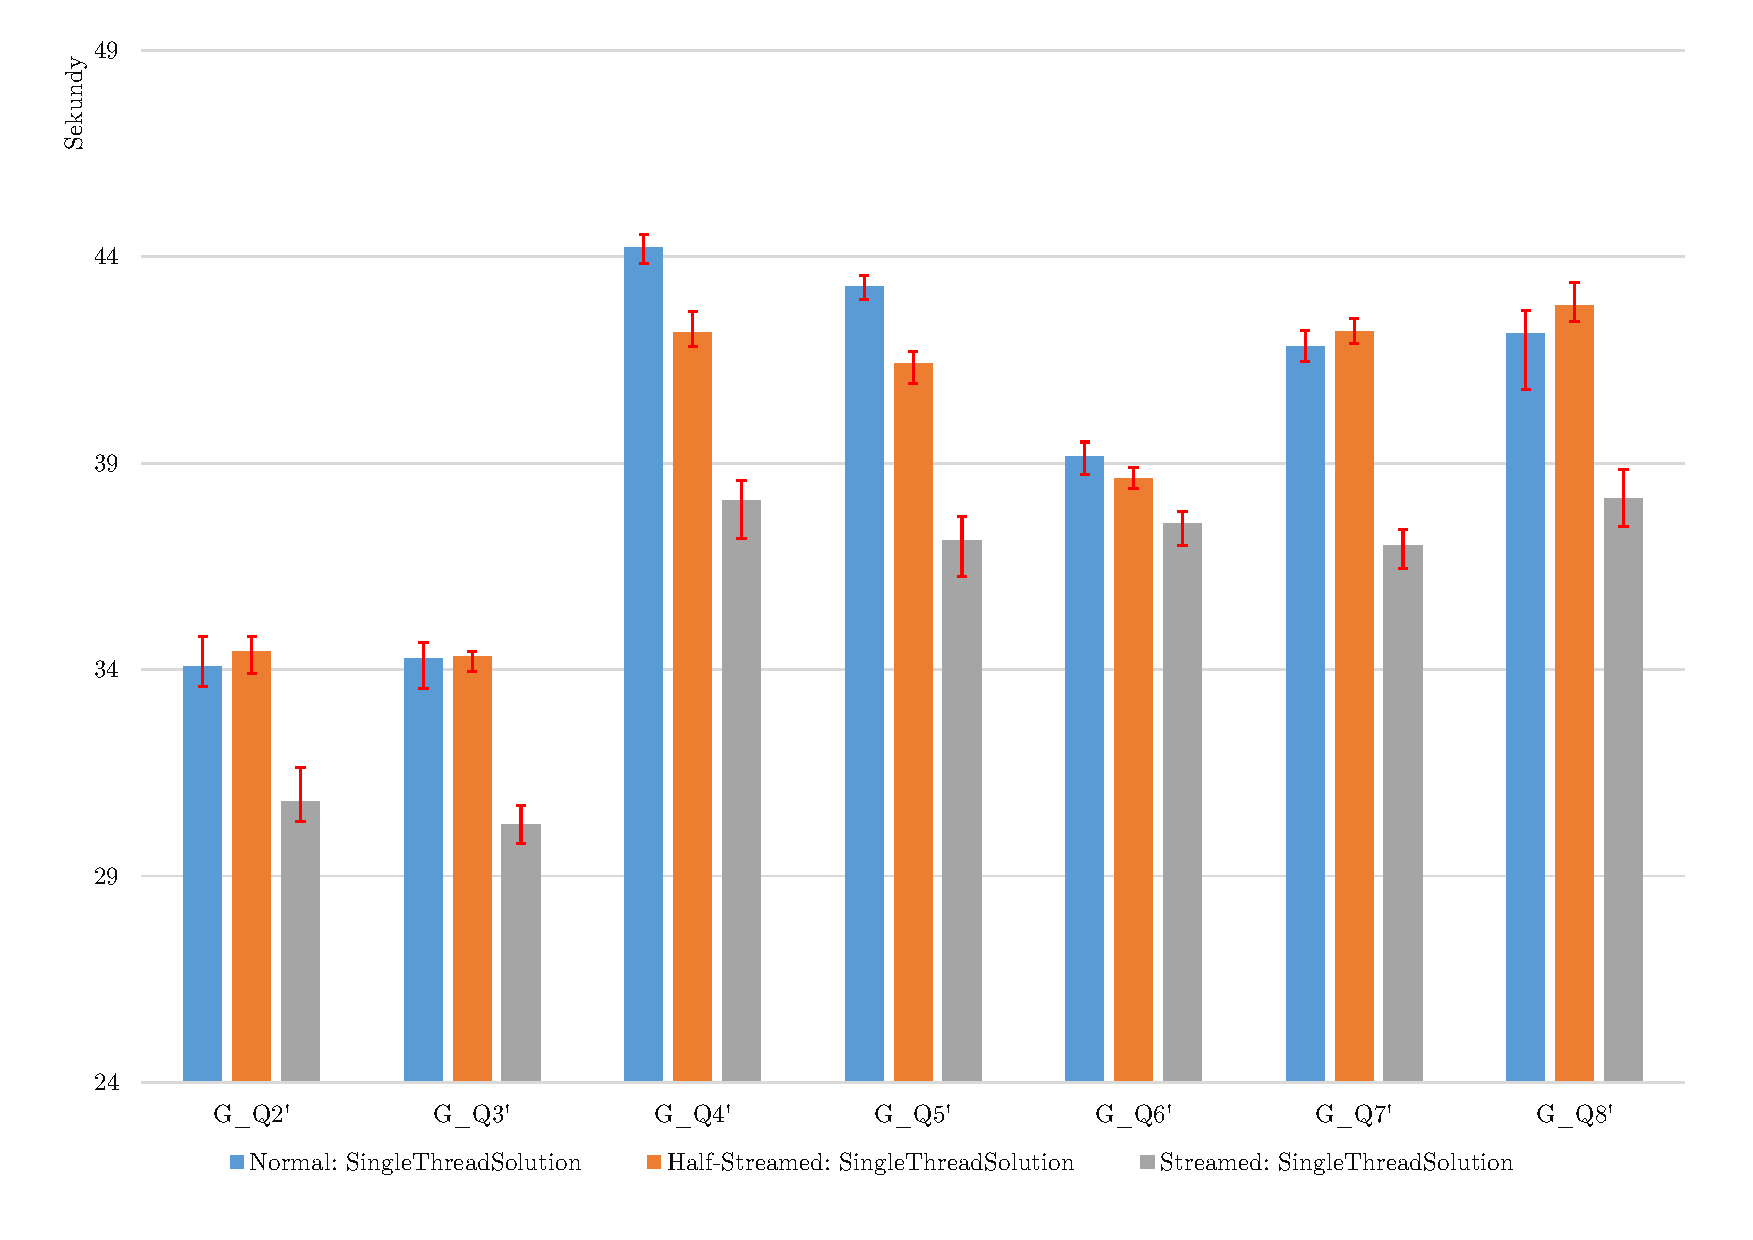
\includegraphics[width=\linewidth]{../img/webberkstanGroupBySTNoAgg.pdf}\centering
\caption{Doba vykonání dotazů Group by bez agr. funkcí pro graf WebBerkStan (sekce \ref{tab.grafBase}). Běh v jednom vláknu. Počet seskupovaných výsledků je 222498869.}
\label{figure.webberkstanGroupBySTNoAgg}
\end{figure}

\begin{figure}[!htp]
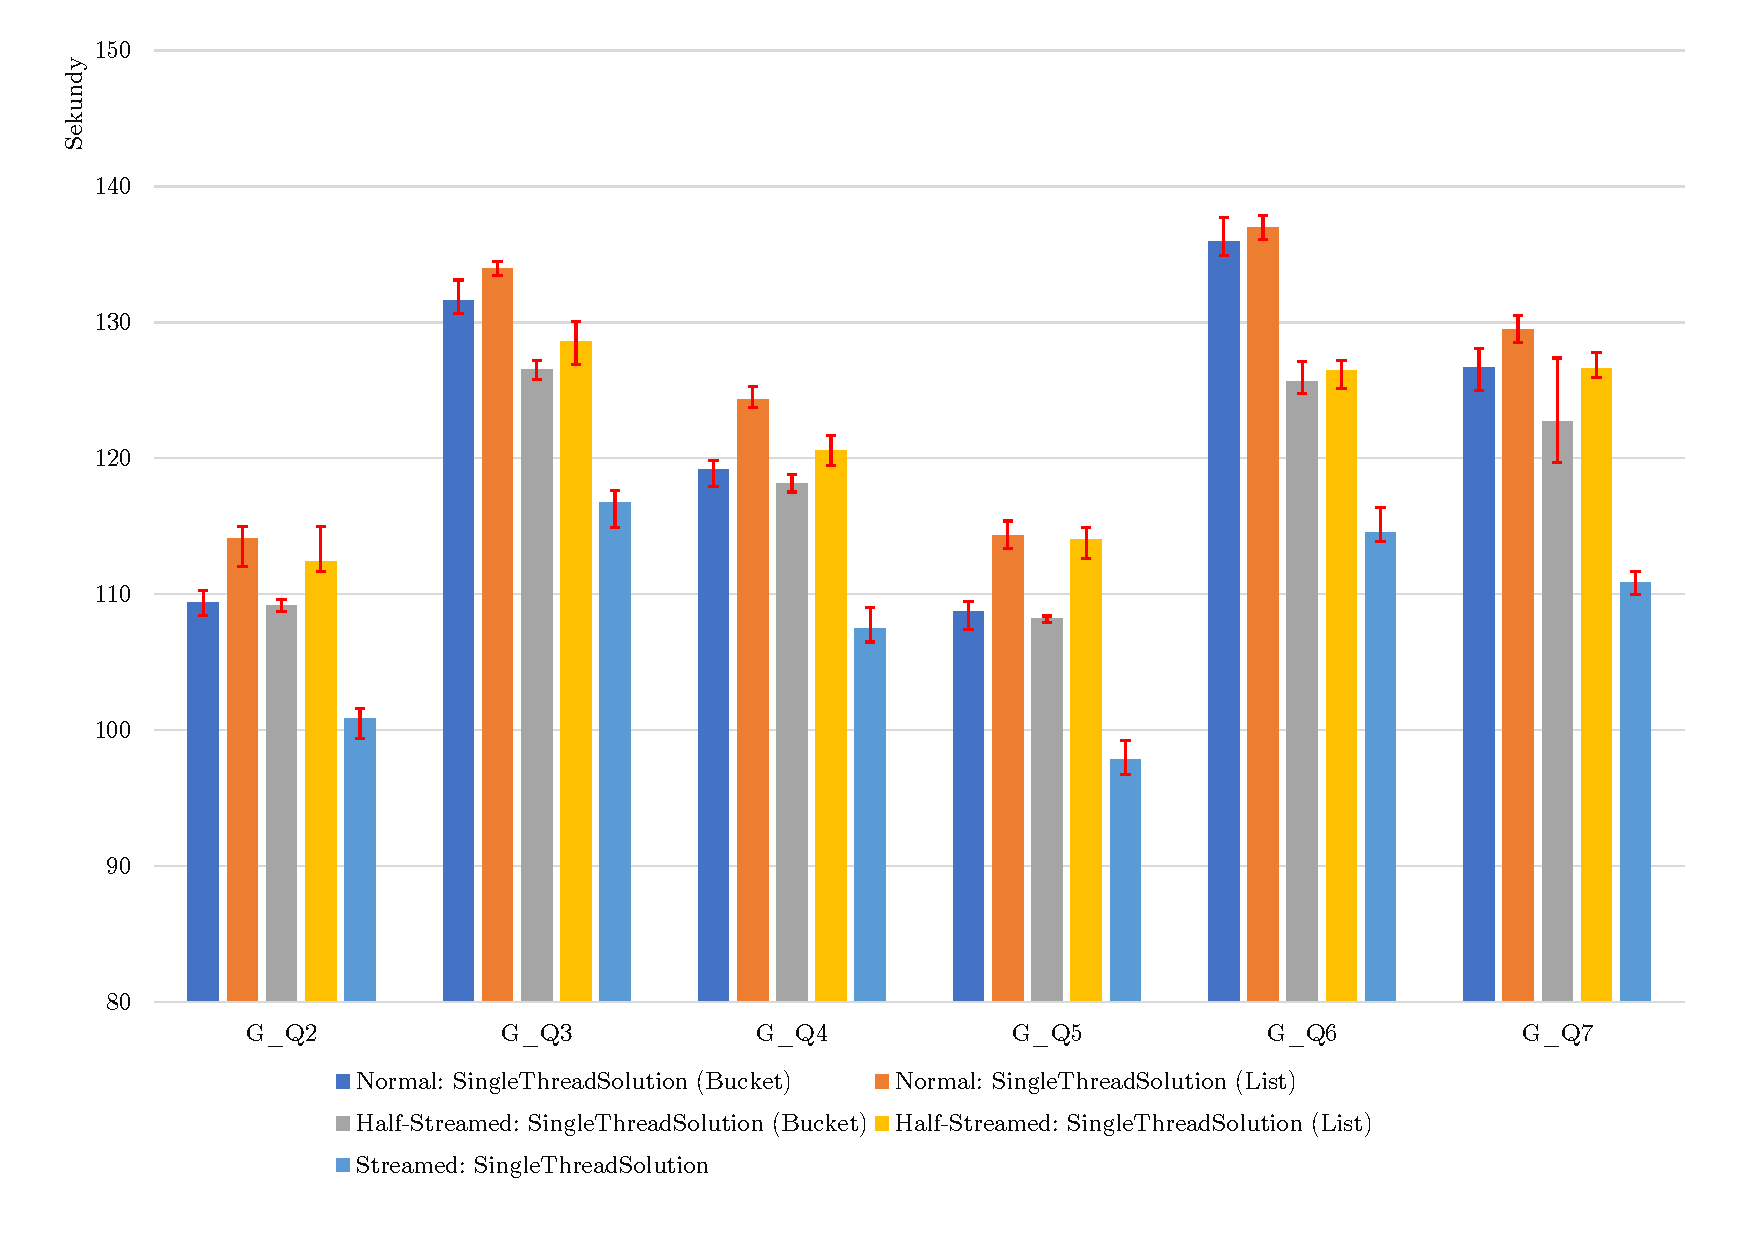
\includegraphics[width=\linewidth]{../img/skitterGroupByST.pdf}\centering
\caption{Doba vykonání dotazů Group by pro graf As-Skitter (sekce \ref{tab.grafBase}). Běh v jednom vláknu. Počet seskupovaných výsledků je 453674558.}
\label{figure.skitterGroupByST}
\end{figure}
\begin{figure}[!htp]
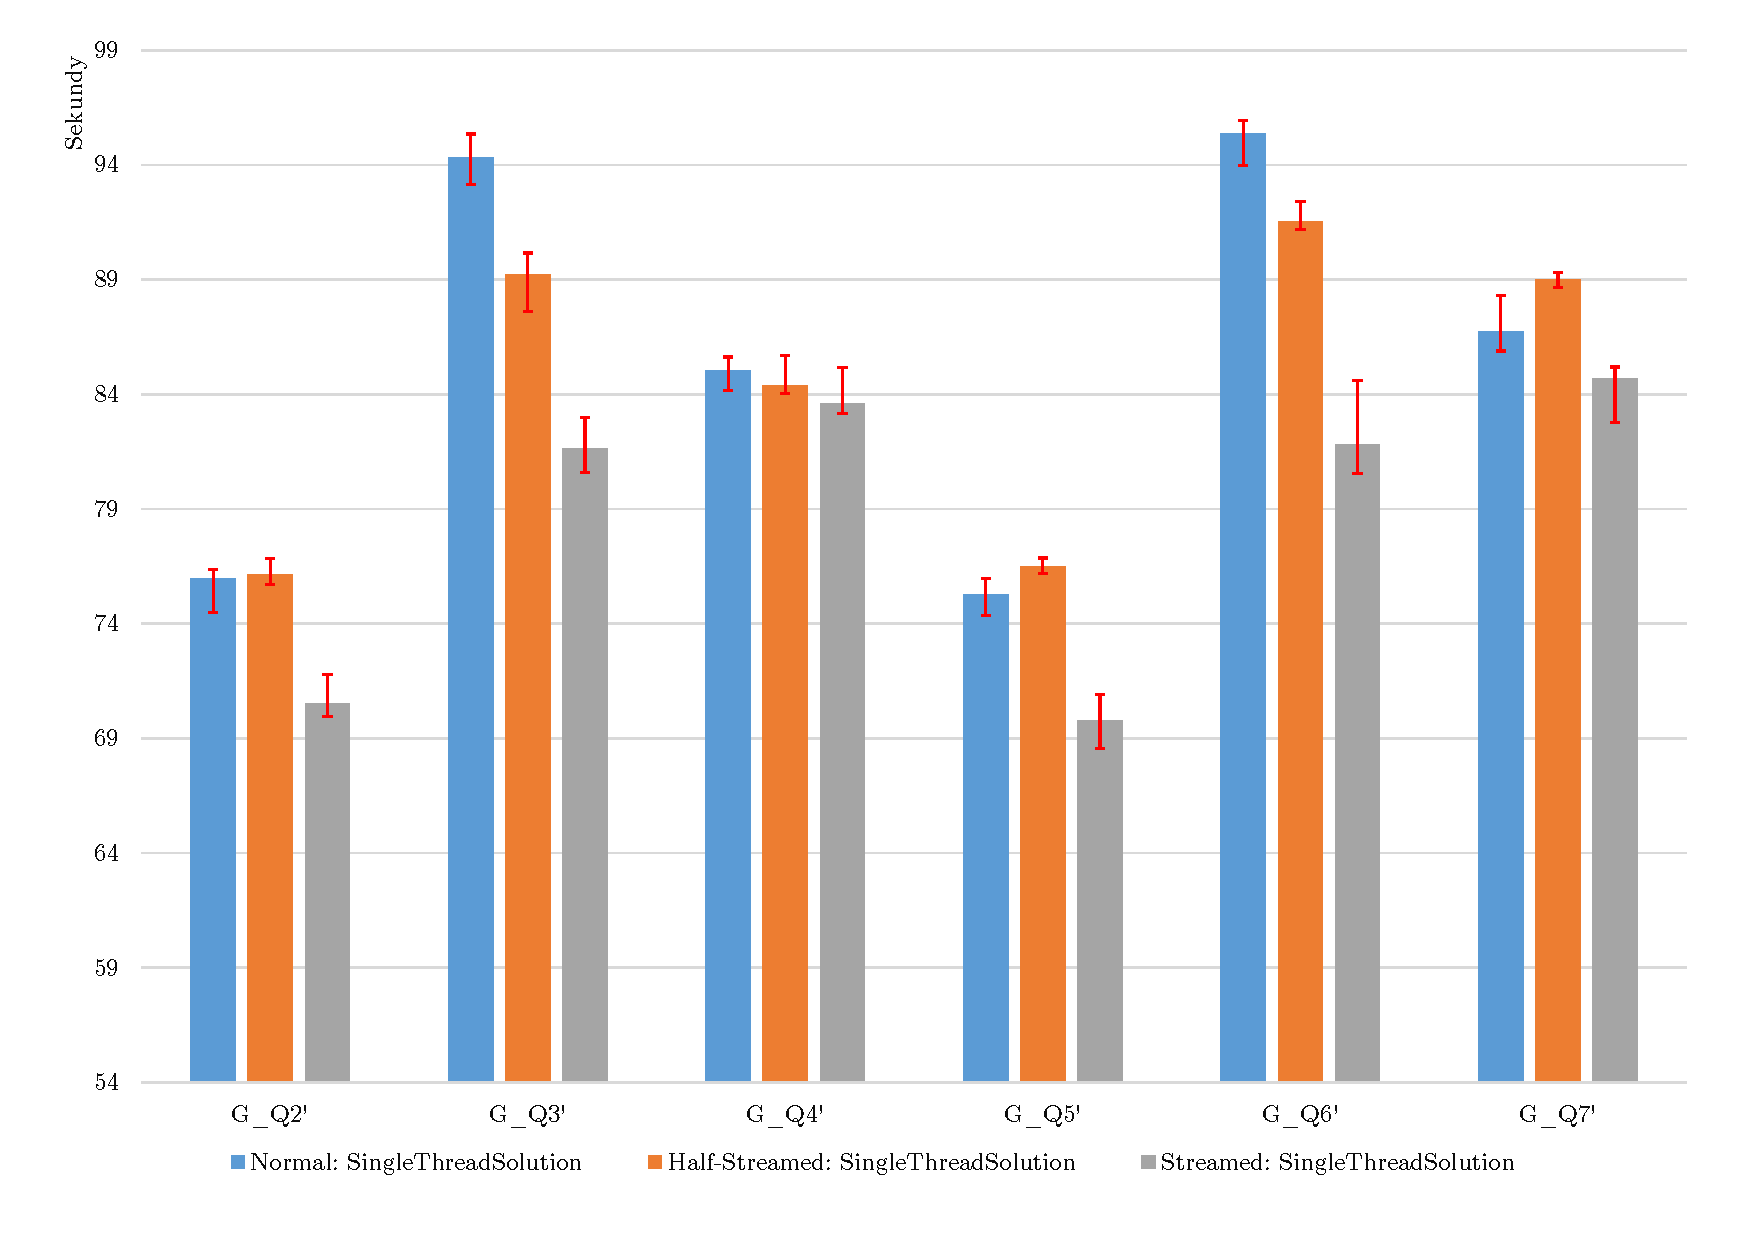
\includegraphics[width=\linewidth]{../img/skitterGroupBySTNoAgg.pdf}\centering
\caption{Doba vykonání dotazů Group by bez agr. funkcí pro graf As-Skitter (sekce \ref{tab.grafBase}). Běh v jednom vláknu. Počet seskupovaných výsledků je 453674558.}
\label{figure.skitterGroupBySTNoAgg}
\end{figure}

Na obrázcích \ref{figure.amazonGroupByST}, \ref{figure.webberkstanGroupByST} a \ref{figure.skitterGroupByST} vidíme výsledky Group by pro běh v jednom vlákně.
Výsledky na obrázcích \ref{figure.amazonGroupBySTNoAgg}, \ref{figure.webberkstanGroupBySTNoAgg} a \ref{figure.skitterGroupBySTNoAgg} představují dotazy bez agregačních funkcí v části Select.
Dvojice dotazů G\_Q4/G\_Q5, G\_Q2/G\_Q3 a G\_Q6/G\_Q7/G\_Q8 jsou pouze mírně rozličná a můžeme u nich vidět konzistenci výsledků pro použité grafy.
Řešení vykonávající Group by v průběhu vyhledávání překonávají Normal řešení.
S růstem počtu výsledku se rozdíly mezi módy prohlubují. 
Například, zrychlení Streamed řešení je znatelnější u grafu As-Skitter než u grafu Amazon0601. 

Obecně nejznačnější zrychlení nastává u Streamed řešení, kdy není použita tabulka výsledků.
Velice mírné zrychlení můžeme vidět u Half-Streamed řešení, které ukládá jen reprezentanty skupiny.
U všech dotazů bez agregačních funkcí, kromě G\_Q4$'$/G\_Q5$'$, nastávají situace, kdy Half-Streamed řešení je pomalejší než Normal.
U grafu Amazon0601 nastává stejná situace pro G\_Q3, G\_Q6 a pro každý graf G\_Q8.
Situaci jsme neočekávali.
Vysvětlujeme si ji následovně.
Half-Streamed řešení používá při zpracování výsledku položku tabulky \verb+temporaryRow+, do které přesouvá pointr na pole výsledků.
Skrze danou položku pak následně přistupuje k výsledku při vkládání do mapy. 
Na dané přesouvání se můžeme dívat jako na kopírovaní jedné proměnné do tabulky.
Při úspěšném vložení nastane navíc překopírování výsledků do pravé tabulky.
Což odpovídá větší režii na zpracování výsledku než u Normal řešení.
Proto vídíme pokles rychlosti a celkově jen mírné zrychlení u Half-Streamed řešení v jiných případech.
Největší skok pak právě nastává v dotazech G\_Q4/G\_Q4$'$ a G\_Q5/G\_Q5$'$, kdy se ukládají dvě proměnné.
Tedy samotná řežie Normal řešení je značně pomalejší, protože musí ukládat vždy dvě proměnné, zatímco Half-Streamed jen přesouvá pointr.
Zajímavé je, že dané situace nastávají u dotazů bez agregačních funkcí, přestože všechna řešení pro jejich reprezentaci používají stejné funkce a struktury (List/Bucket).
Předpokládali bychom tedy stejnou situaci i na ostatních (větších) grafech.
Absenci jevu neumíme plně objasnit.

Na největším grafu platí, že použité ukládání List je pomalejší než Bucket, kvůli indirekci navíc.
Na menších grafech rozdíly ustupují a dokonce nastavají situace, kdy je List rychlejší. 
Přesněji u dotazů G\_Q4 a G\_Q5.
Přehození rolí si u nich vysvětlujeme overheadem za množství vytvářených polí (tj. hodně alokací, málo přístupů), které se vyrovná použité indirekci.
Na grafu Amazon0601 u  G\_Q4 a G\_Q5 dotazů je Streamed řešení pomalejší než Half-Streamed (List), protože také vytváří pole jako Bucket řešení (viz implementace TODO).
U dalších grafů je pak počet vytváření polí mnohonosábně menší než počet přístupů k nim.

Z výsledků můžeme vyvodit, že vylepšená řešení pro single thread Group by jsou výhodnější z hlediska rychlosti vykonávání než řešení Normal. 
Nyní přejdeme k výsledkům paralelizace.

%%%%%%%%%%%%%%%%%%%%%%%%%%%%

Paralelní řešení používají doposud zmíněná značení.
Global řešení seskupuje výsledky globálně pomocí paralelní mapy (\verb+ConcurrentDictionary+).
Two-Step řešení seskupuje výsledky nejdříve lokálně pomocí mapy a následném mergi do paralelní mapy.
LocalGroupByLocalTwoWayMerge řešení seskupuje lokálně a následně merguje výsledky vláken po dvojicích. 
Toto Mergování si můžeme představit jako binární strom. Listy jsou výsledky vláken a vnitřní vrcholy jsou akce mergování.
Výsledky paralelizování jsou zobrazeny na obrázcích \ref{figure.amazonGroupByPar}, \ref{figure.webberkstanGroupByPar} a \ref{figure.skitterGroupByPar}.
Obrázky \ref{figure.amazonGroupByParNoAgg}, \ref{figure.webberkstanGroupByParNoAgg} a \ref{figure.skitterGroupByParNoAgg} obsahují výsledky dotazů bez agregačních funkcí.
\bigskip

\begin{figure}[!htp]
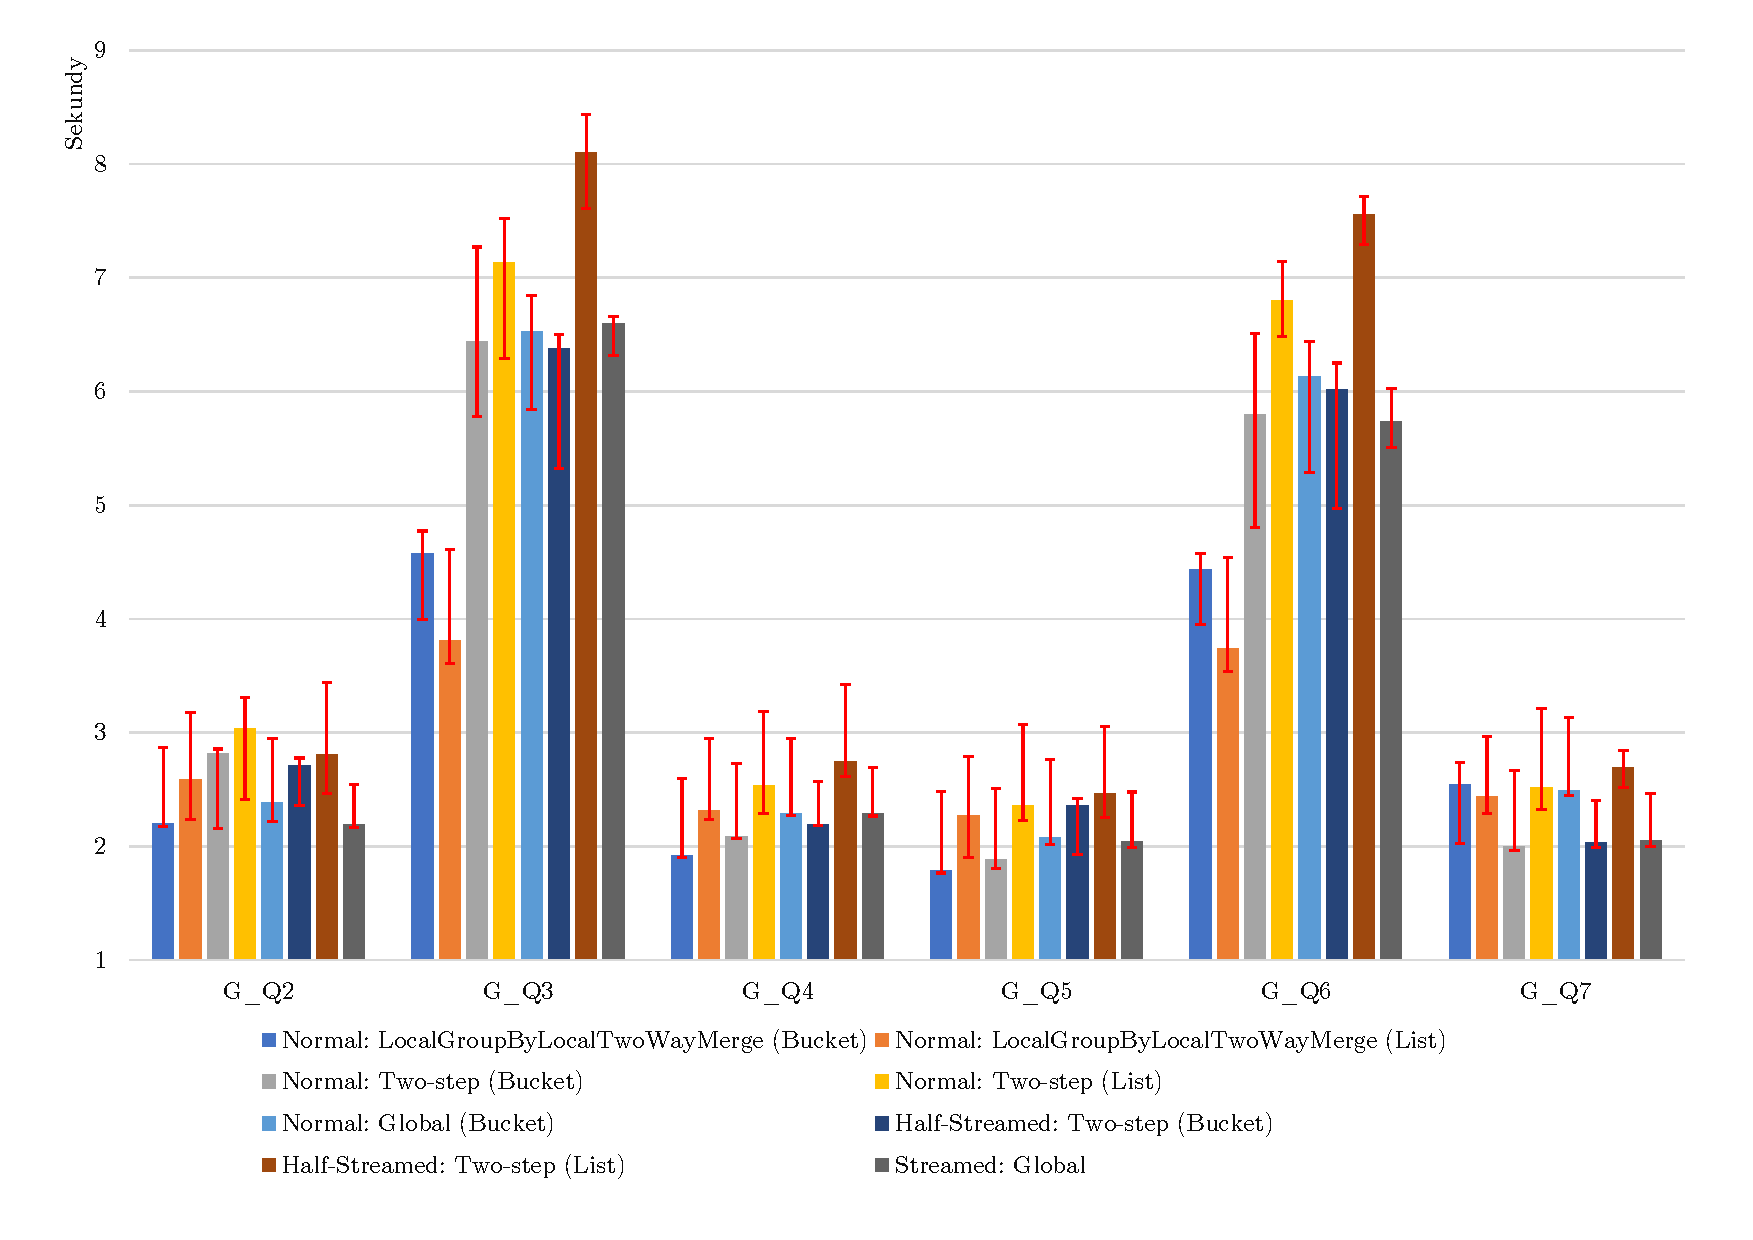
\includegraphics[width=\linewidth]{../img/amazonGroupByPar.pdf}\centering
\caption{Doba vykonání dotazů Group by pro graf Amazon0601 (sekce \ref{tab.grafBase}). Běh osmi vláken. Počet seskupovaných výsledků je 32373599.}
\label{figure.amazonGroupByPar}
\end{figure}
\begin{figure}[!htp]
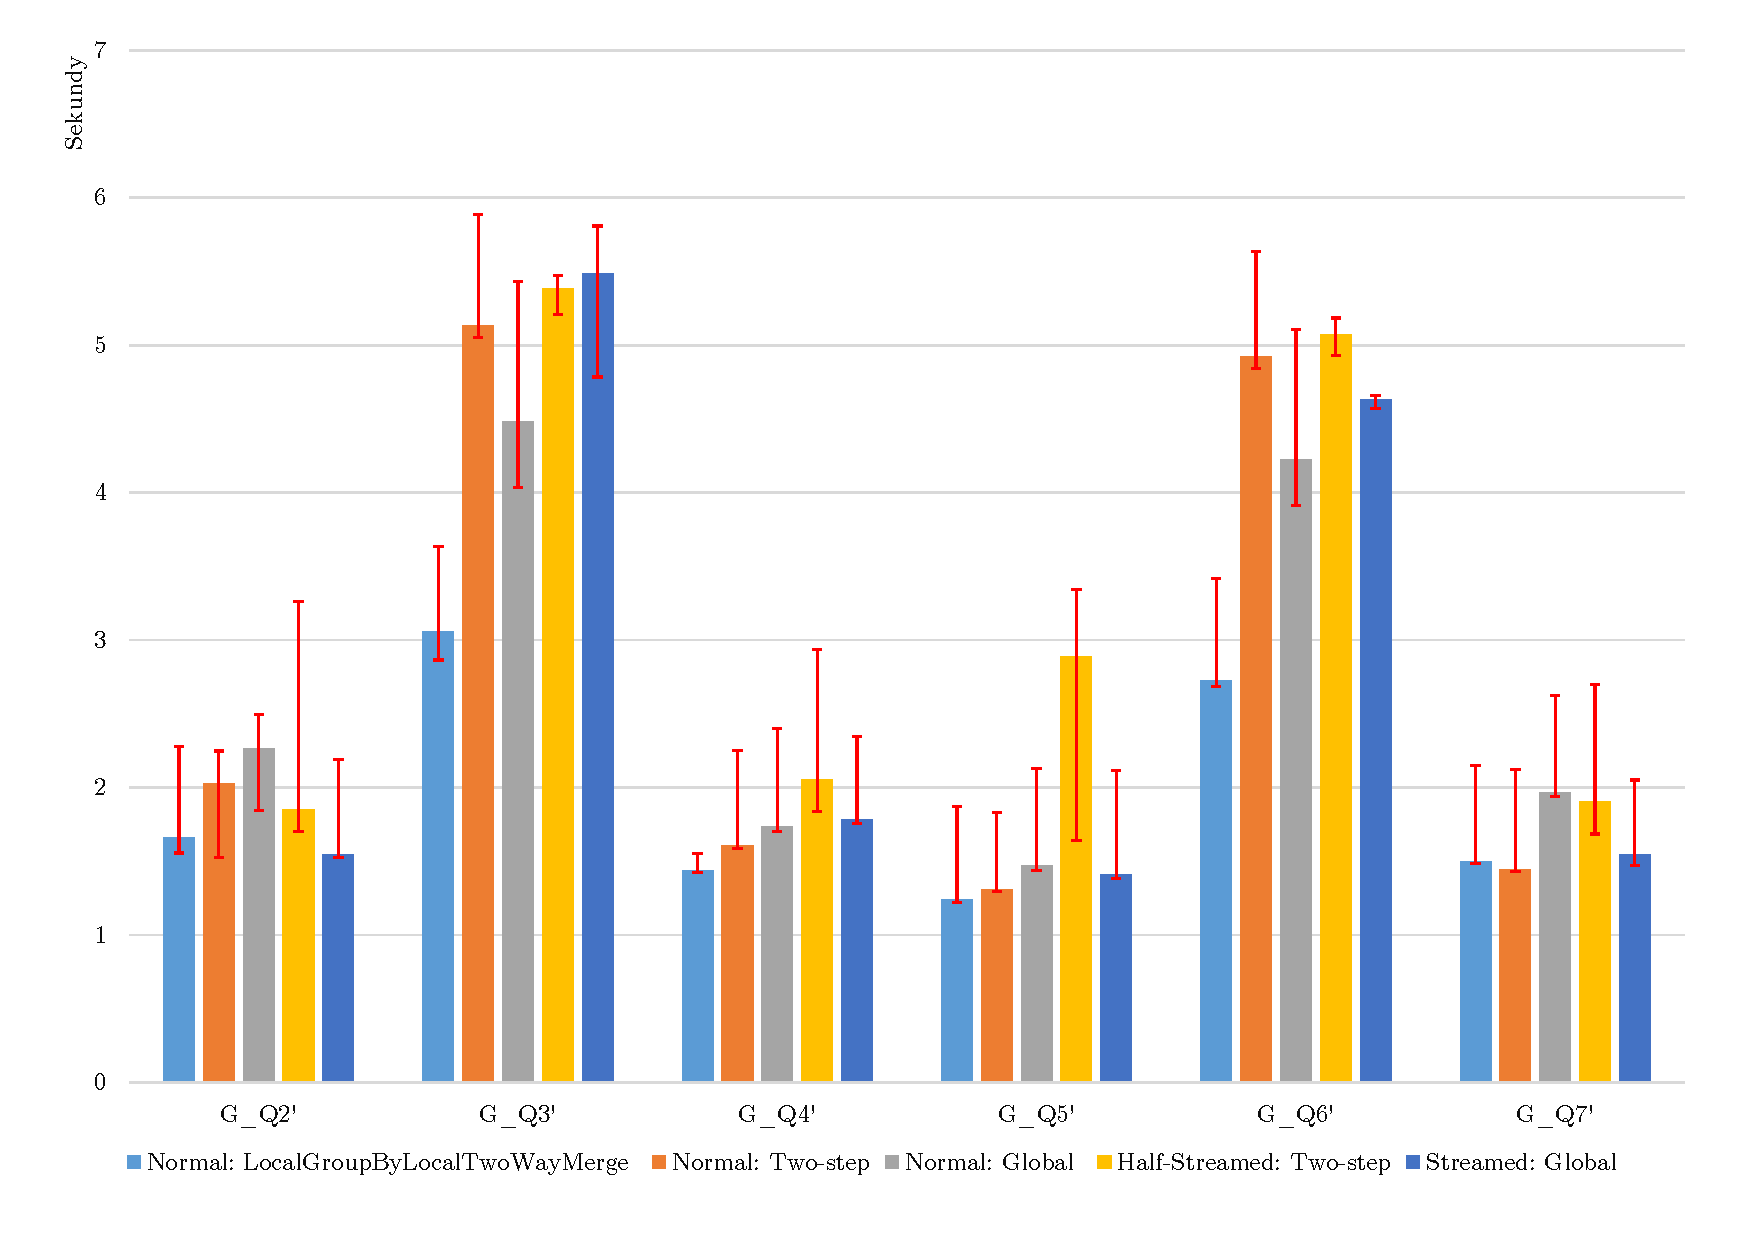
\includegraphics[width=\linewidth]{../img/amazonGroupByParNoAgg.pdf}\centering
\caption{Doba vykonání dotazů Group by bez agr. funkcí pro graf Amazon0601 (sekce \ref{tab.grafBase}). Běh osmi vláken. Počet seskupovaných výsledků je 32373599.}
\label{figure.amazonGroupByParNoAgg}
\end{figure}

\begin{figure}[!htp]
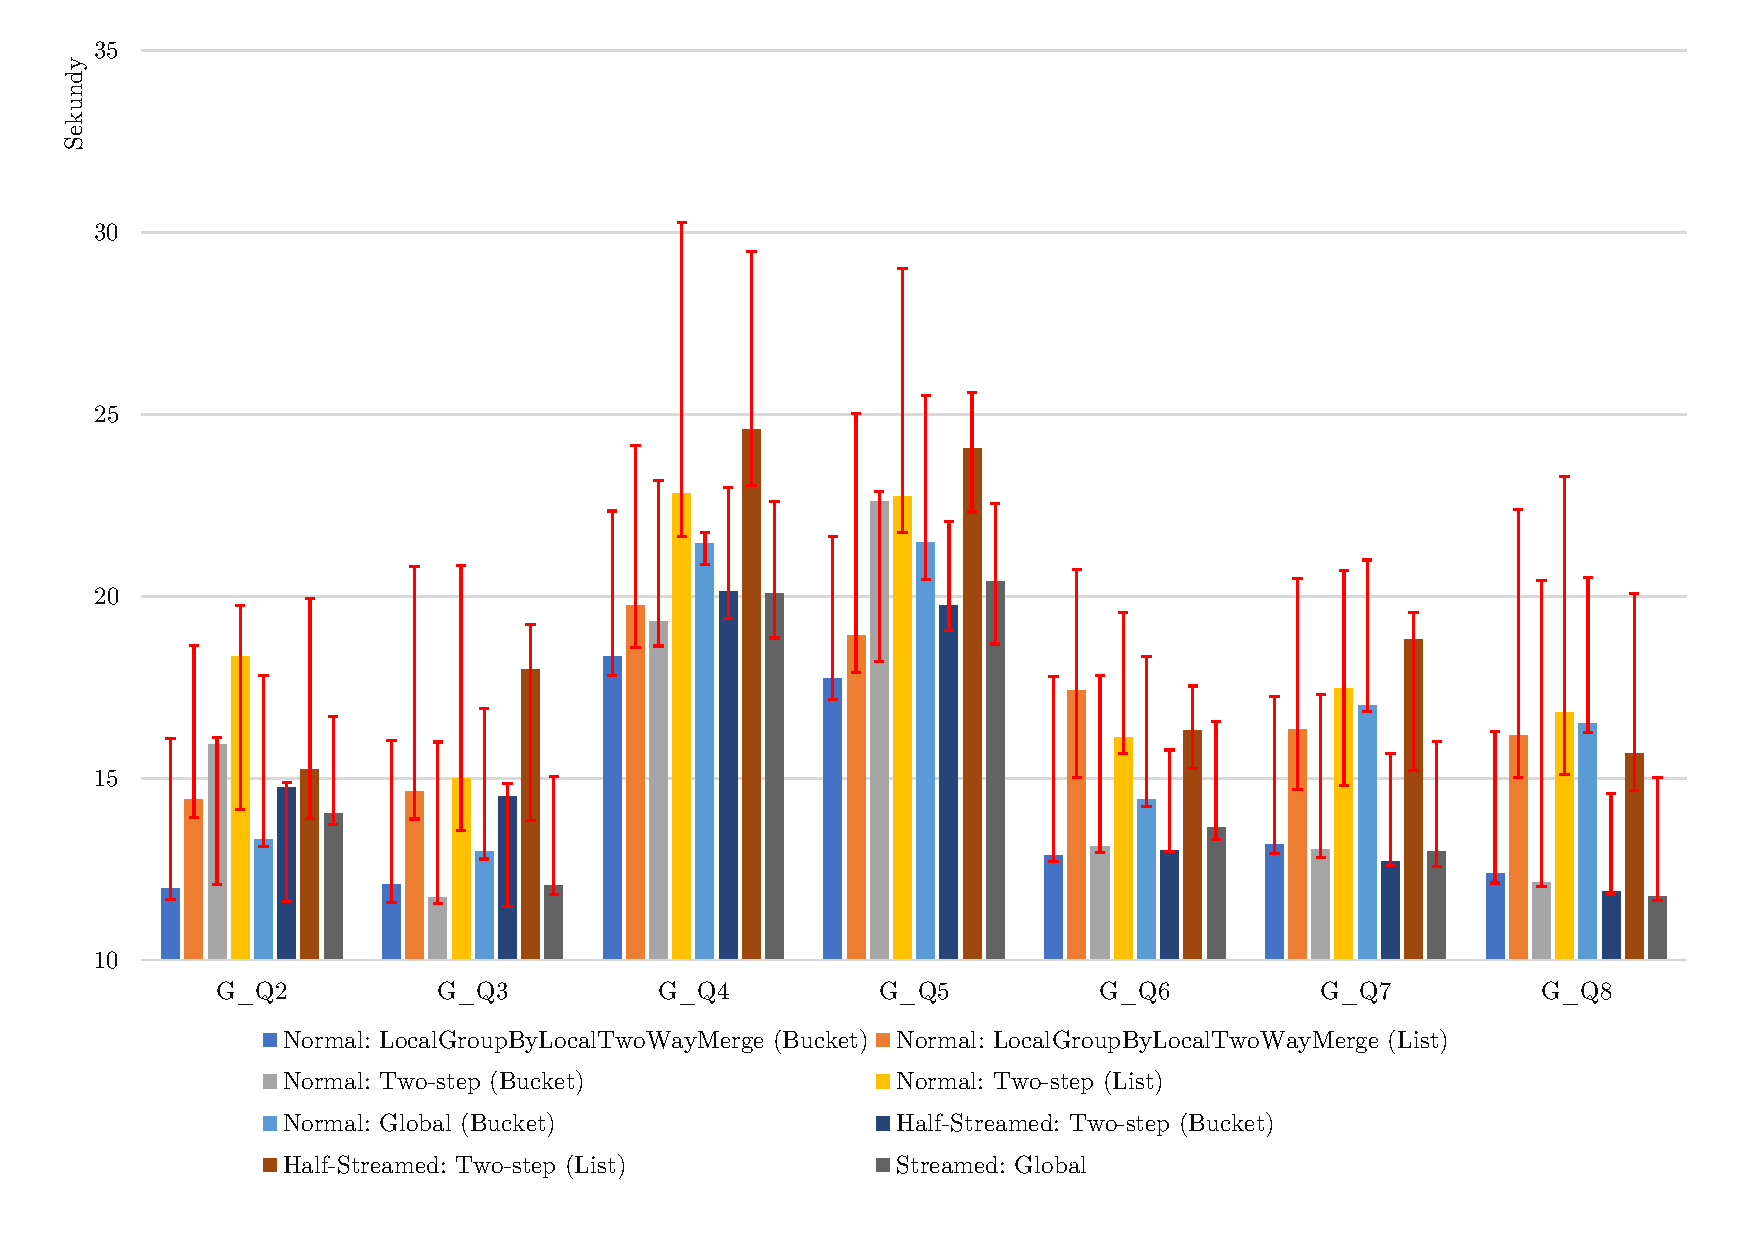
\includegraphics[width=\linewidth]{../img/webberkstanGroupByPar.pdf}\centering
\caption{Doba vykonání dotazů Group by pro graf WebBerkStan (sekce \ref{tab.grafBase}). Běh osmi vláken. Počet seskupovaných výsledků je 222498869.}
\label{figure.webberkstanGroupByPar}
\end{figure}
\begin{figure}[!htp]
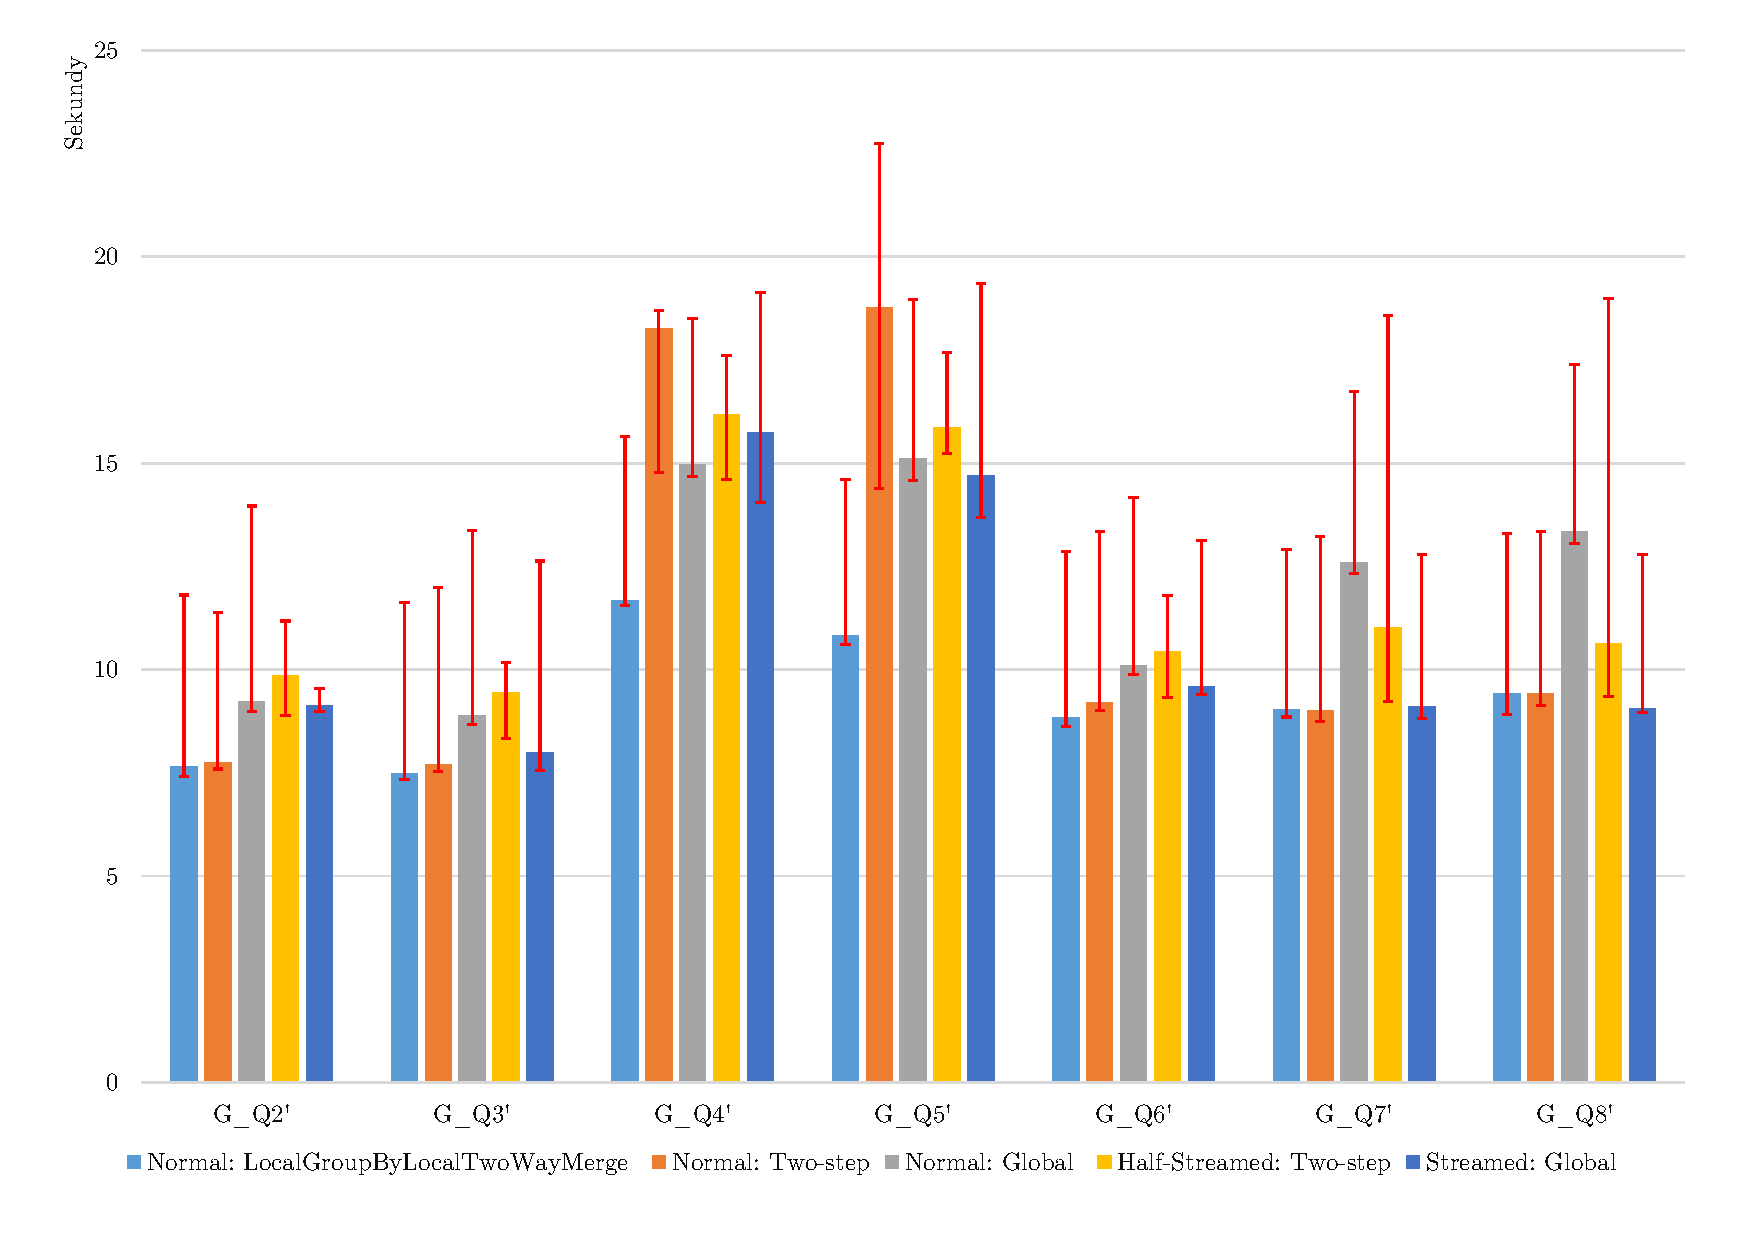
\includegraphics[width=\linewidth]{../img/webberkstanGroupByParNoAgg.pdf}\centering
\caption{Doba vykonání dotazů Group by bez agr. funkcí pro graf WebBerkStan (sekce \ref{tab.grafBase}). Běh osmi vláken. Počet seskupovaných výsledků je 222498869.}
\label{figure.webberkstanGroupByParNoAgg}
\end{figure}

\begin{figure}[!htp]
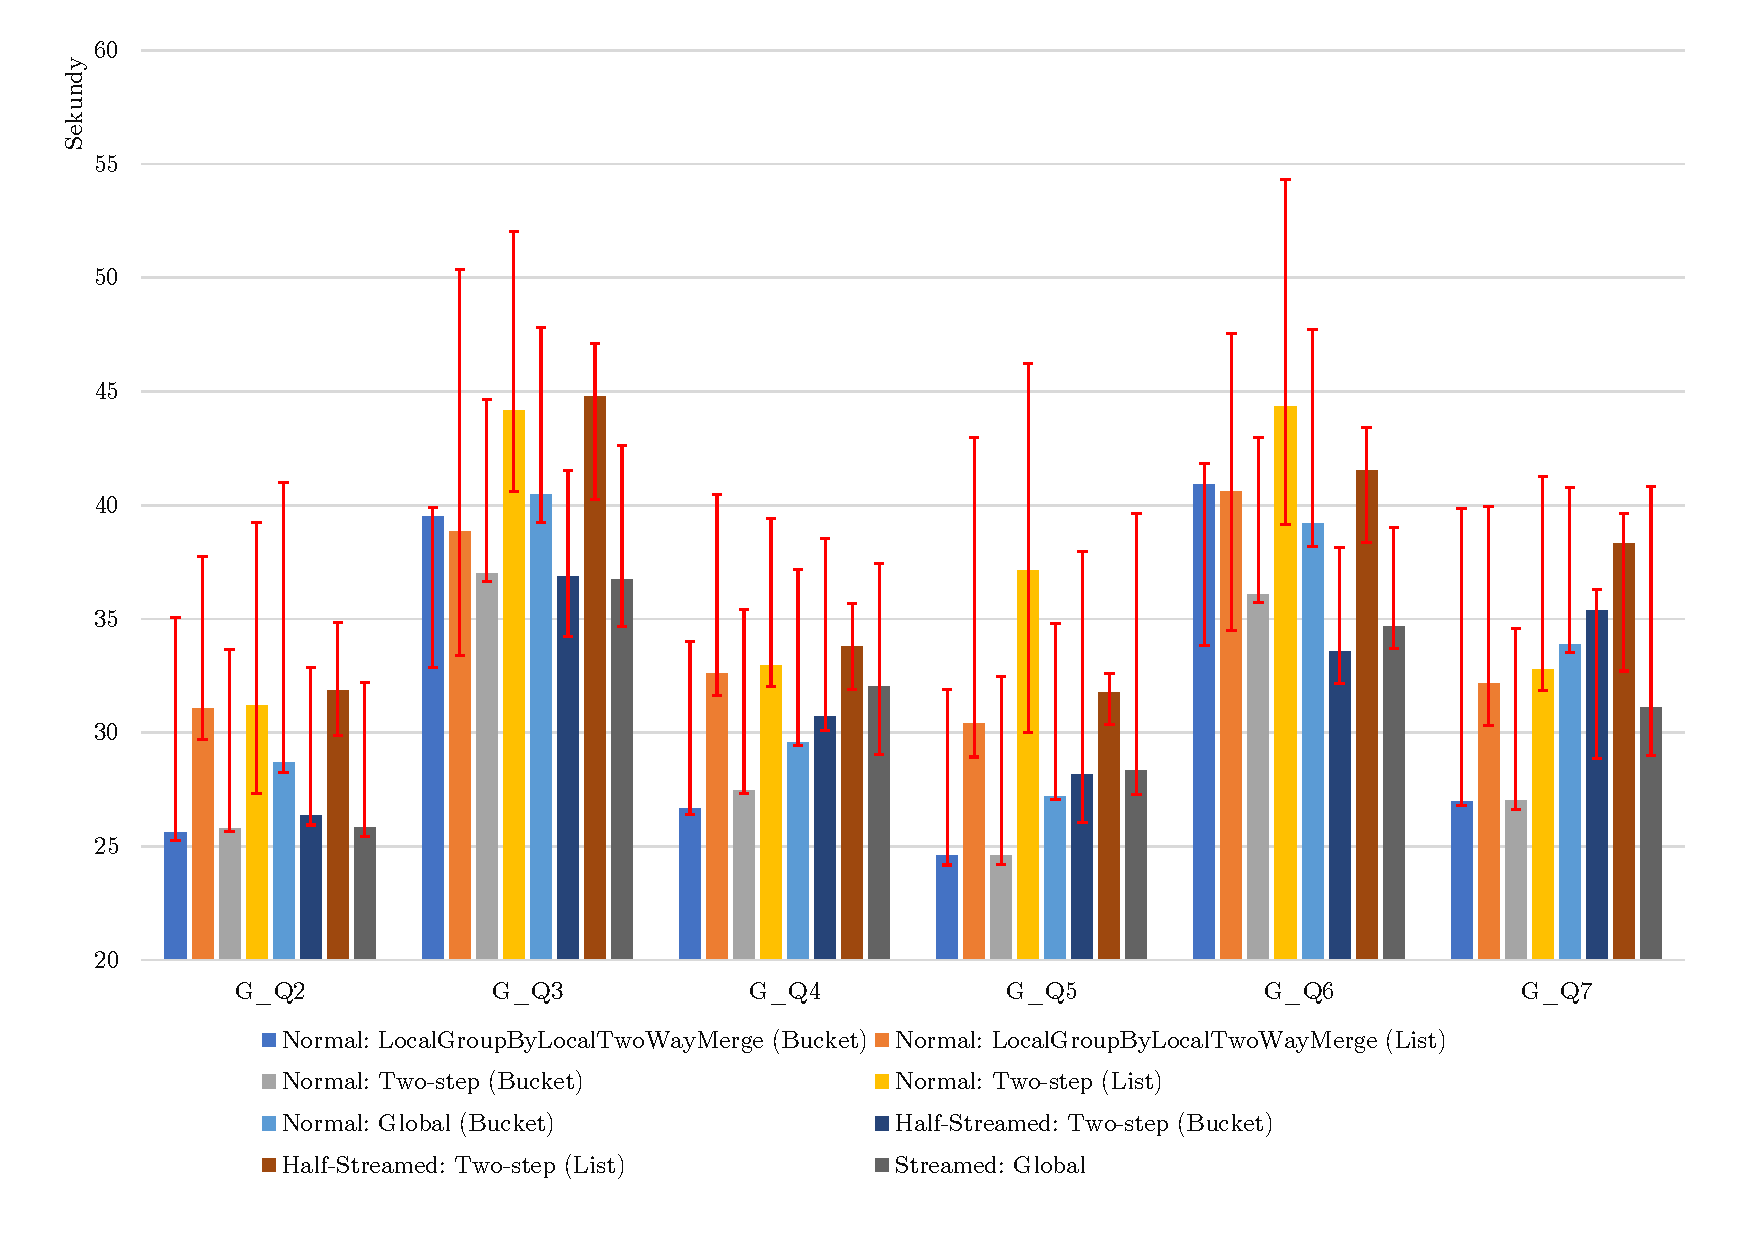
\includegraphics[width=\linewidth]{../img/skitterGroupByPar.pdf}\centering
\caption{Doba vykonání dotazů Group by pro graf As-Skitter (sekce \ref{tab.grafBase}). Běh osmi vláken. Počet seskupovaných výsledků je 453674558.}
\label{figure.skitterGroupByPar}
\end{figure}
\begin{figure}[!htp]
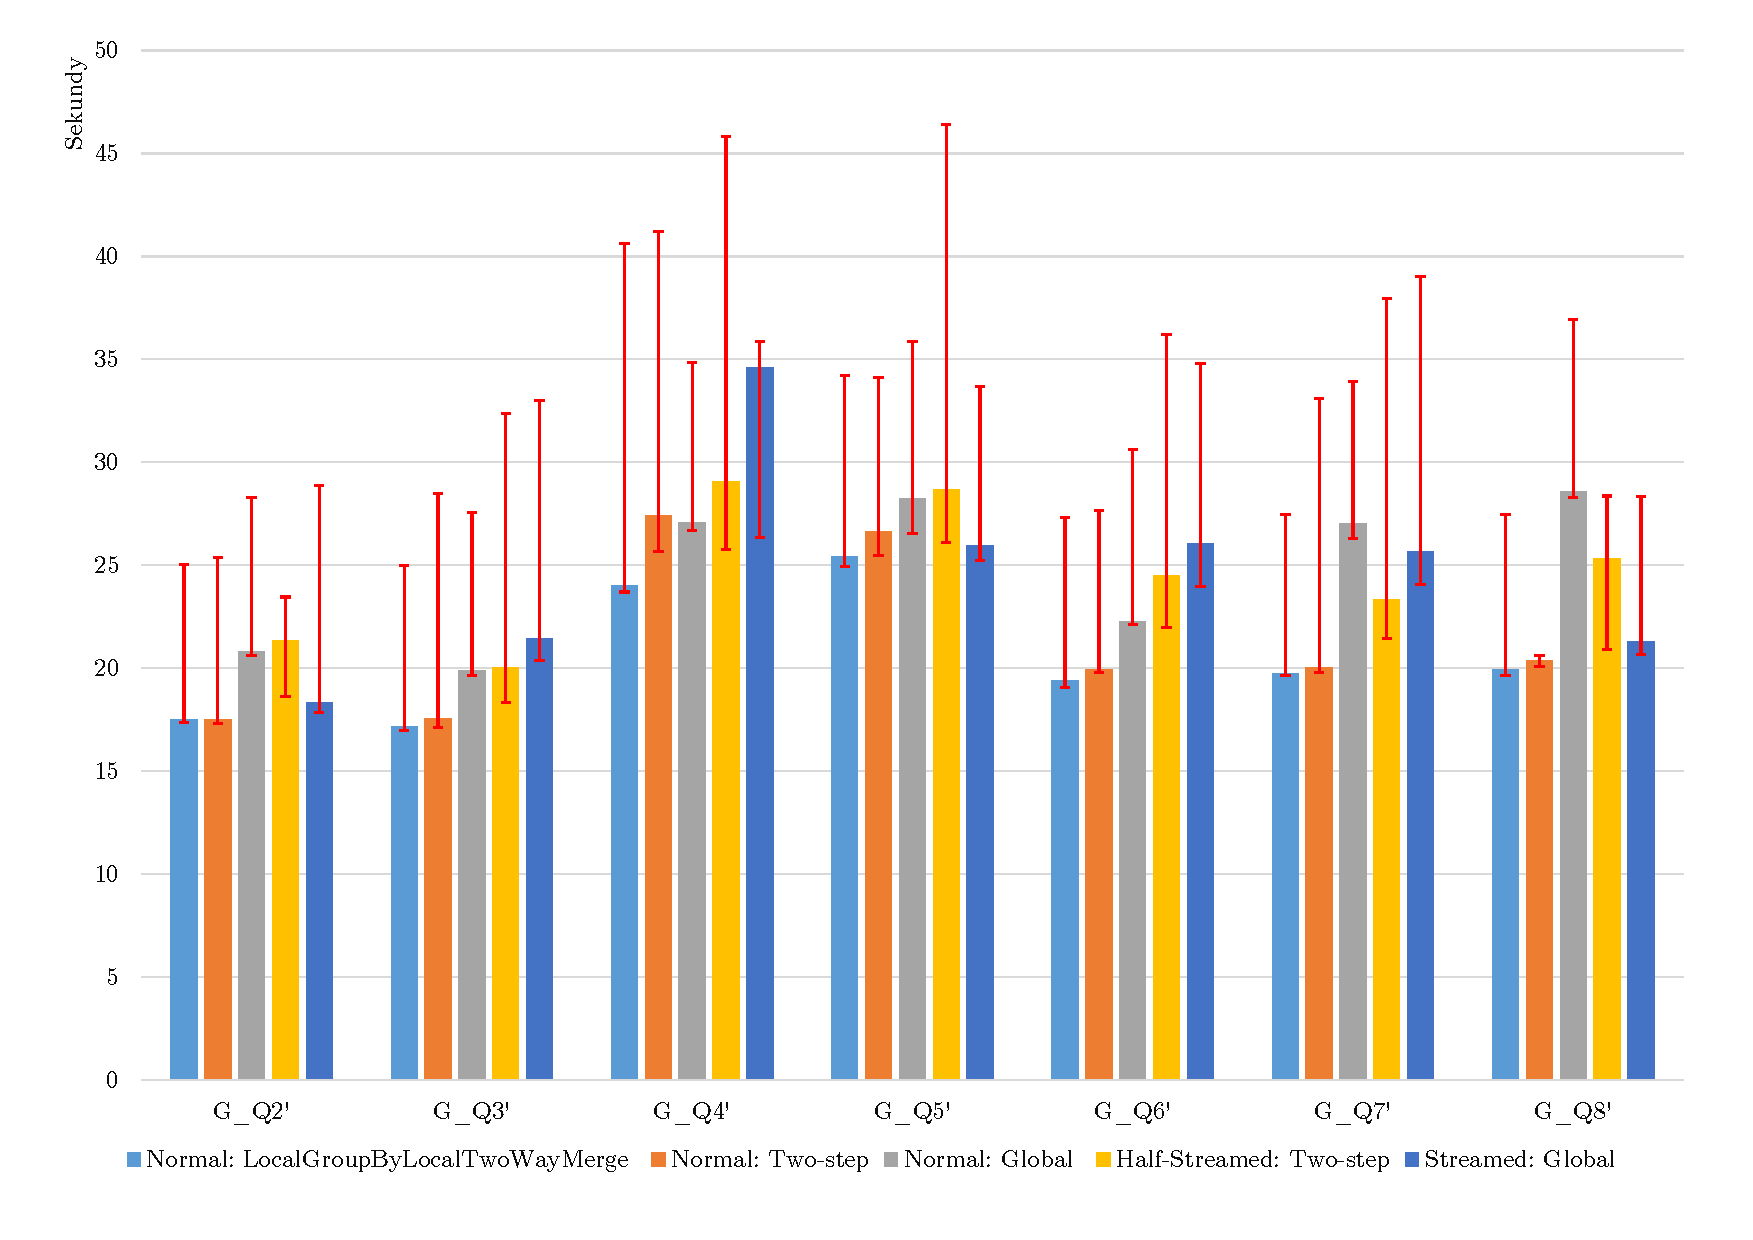
\includegraphics[width=\linewidth]{../img/skitterGroupByParNoAgg.pdf}\centering
\caption{Doba vykonání dotazů Group by bez agr. funkcí pro graf As-Skitter (sekce \ref{tab.grafBase}). Běh osmi vláken. Počet seskupovaných výsledků je 453674558.}
\label{figure.skitterGroupByParNoAgg}
\end{figure}

Byli jsme překvapeni, že vylepšená řešení se mnohdy nevyrovnala původním řešením.
Streamed řešení, ačkoliv bylo nejrychlejší v jednovláknovém běhu, tak zde se pouze vyrovnalo Normal řešením a nebo bylo pomalejší.
Danou situaci si vysvětlujeme synchronizací. 
Prvni vrstva synchronizace nastává u přistupu k paralelní mapě a čtení/vložení záznamu.
Po získání \verb+value+ z mapy následuje druhá vrstva, která obsahuje volání thread-safe funkcí pro výpočet agregovaných hodnot pro danou skupinu.
Z obrázků \ref{figure.amazonGQ1Par}, \ref{figure.webberkstanGQ1Par} a \ref{figure.skitterGQ1Par} (Streamed řešení) jsme viděli cenu za synchronizaci na agregačních funkcích při přístupu osmi vláken.
Pro představu pouhé režie paralelní mapy jsme otestovali overhead zvlášť čtení a vložení \verb+ConcurrentDictionary<int, int>+ vůči \verb+Dictionary<int,int>+ pro jedno vlákno.
Následuje příklad kódu použitého při testu:
\begin{code}
Random ran = new Random(100100);
Stopwatch timer = new Stopwatch();
Dictionary<int, int> map = new Dictionary<int, int>();
ConcurrentDictionary<int, int> parMap = 
    new ConcurrentDictionary<int, int>();
...
// Insert test. Assuming the maps are empty.
for (int i = 0; i < 1_000_000; i++)
{
    var val = ran.Next();
    // Based on the used map choose (1) or (2).
    (1) if (!map.TryGetValue(val, out int value)) map.Add(val, i);
    (2) var tmp = parMap.GetOrAdd(val, i);
}
...
// Read test. Assuming the maps contain keys from 0 to 1_000_000.
for (int i = 0; i < 100_000_000; i++)
{
    var val = ran.Next(0, 1_000_000);
    // Based on the used map choose (1) or (2).
    (1) if (!map.TryGetValue(val, out int value));
    (2) var tmp = parMap.GetOrAdd(val, val);
}
\end{code}


\begin{table}[!htb]
\centering
\begin{tabular}{lrrr}
\toprule
\mc{Test} & \mc{\textbf{Dictionary}} & \mc{\textbf{ConcurrentDictionary}} & \mc{\textbf{Poměr}} \\
\midrule
Insert 1000000 & 165 & 667 & 4,04 \\
Insert 10000000  & 2476 & 11272 & 4,55 \\
Read 100000000  & 19002 & 21516 & 1,13 \\
\bottomrule
\end{tabular}

\caption{Výsledky testování map v milisekundách. Běh v jednom vlákně. Měření dle kódu výše. Generování prvků pomocí třídy Random se seedem 100100. Měřeno pomocí třídy Stopwatch. Výsledek zvolen jako průměr pěti měření. Test Insert $n$ provádí vkládání $n$ náhodně vygenerovaných prvků do prázdné mapy. Test Read $n$ provádí $n$ čtení z rozsahu 0 až 1000000. Poměr je roven podílu času paralelní mapy a mapy.}
\label{tab.mapsInsert}
\end{table}

\clearpage

Tabulka naměřených hodnot testování (tab.mapsInsert) ukazuje, že pouhé vkládání náhodně generovaných prvků do paralelní mapy trvá průměrně 4x déle.
Samostatné čtení náhodně generovaných hodnot, které existují v mapě, je průměrně o 13\% pomalejší.
Proto vidíme u Streamed řešení postupné vyrovnání pro dotazy G\_6/G\_6$'$ až G\_8/G\_8$'$, kde v G\_8/G\_8$'$ dochází k nejmenší tvorbě skupin a častému čtení.
Obecné zpomalení je zřetelné u řešení používající paralelní mapu.
Streamed řešení vůči jeho podobnému protějšku Normal: Global je místy pomalejší pozorujeme-li dolní hranice ve dvou grafech.
První je graf As-Skitter u dotazů  G\_3/G\_3$'$ a  G\_6/G\_6$'$.
Druhý graf je Amazon0601 na dotazech G\_4/G\_4$'$ a  G\_5/G\_5$'$.
Myslíme si, že se jedná o specifické situace pro dané grafy a nedokážeme je plně zodpovědět, jelikož navzájem a pro graf WebBerkStan nenastávají.

Můžeme zde aplikovat výsledky z single-thread řešení pro řešení Normal: Two-Step proti Half-Streamed: Two-Step.
Half-Streamed řešení je zde opět pomalejší než Normal řešení nebo jsou vyrovnané.
Dále zde opět vidíme zpomalení implementace List vůči Bucket, které jsme viděli u single-thread řešení.
Situace při které je List rychlejší nastávala pro dotazy G\_Q4 a G\_Q5 na grafu Amazon0601 a WebBerkStan.
Nyní nastává pouze pro graf Amazon0601 s řešením Normal: LocalGroupByLocalTwoWayMerge.
Two-step (List) řešení při mergi překopírovává větší množství dat, proto u něj daný jev už nenastává. 

Všem řešením dominuje Normal: LocalGroupByLocalTwoWayMerge, které provádí vše lokálně a ujišťuje nás v předpokladu, že hlavní overhead je způsoben synchronizací.
Například dané řešení vůči Normal: Two-Step. 
Je zde vidět overhead za použití paralelní mapy vůči mergování lokálně po dvojicích, jelikož samotný první krok je totožný pro obě řešení.
Zpomalení Normal: Two-Step je ještě znatelnější pro dotazy G\_Q4/G\_Q4$'$ a G\_Q5/G\_Q5$'$, kdy se vkládá množství skupin do paralelní mapy.

Z výsledků usuzujeme, že vylepšená řešení pro náš případ paralelizace neposkytují z hlediska rychlosti vykonání znatelné výhody oproti stávajícím řešením.
Pro budoucí práci by bylo vhodné udělat podrobnější testování pro rozličné počty použitých vláken a sledovat skalabilitu daných řešení.
Další možný budoucí výzkum může sledovat obecný problém rozdělení dat vláken během vyhledávání. 
Normal přistup rovnoměrně rozděluje množství výsledků pro každé vlákno.
Rozdělení práce vylepšených řešení závísí na počtu vyhledaných výsledků v každém vlákně. 
Aby došlo k rovnoměrnému rozdělení práce tak se každému vláknu přidělují malé skupiny vrcholů k prohledání.
Nicméně, dané řešení nemůže zaručit stoprocentně rovnoměrné rozdělení práce.

\bigskip
\textit{Tímto jsme zakončili prezentaci výsledků. Všechna nasbíraná data použitá k tvorbě grafů je možné nalézt v příloze výsledků benchmarku (\ref{prilohy.grafyVysledky}).}